\documentclass{UoYCSproject}

\usepackage{fullpage}
\usepackage{amsmath}
\usepackage{color}
\usepackage{graphicx}
\usepackage{tikz}
\usepackage{array}
\usepackage{multirow}
\usetikzlibrary{positioning,shapes.geometric}

\title{Towards a Building Modelling Framework: Heuristic-EZ}
\MEng{}
\author{Martin Higgs}
\date{\today}
\supervisor{Iain Bate}
\wordcount{}

\abstract{
    This project aims to establish a framework around which building analytics systems can be built and evaluated. The set of building analytics systems are established as those performing crowd-sourced data gathering, indoor positioning (IPS) and generating automated schematics across an enclosed space. Upon reviewing a number techniques for each component, it was seen that most were disjoint; each operating on an undisclosed data set with a proprietary implementation of both their own techniques and the systems being compared against. 
    
    To remedy this a reference implementation of an IPS based on Microsoft's EZ system was developed to test against the UJIIndoorLoc data set as a common comparison point for future work. During development, a number of unnoted deficiencies were found, documented and resolved and a number of heuristic variants of EZ components were created to handle the larger data sets. Evaluation of these techniques then showed median error values of <10\% of the size of the space (comparable with EZ's evaluation) while making use of markedly less complex algorithms. It is anticipated that this work will be continued with other projects building more variants and techniques around the provided software for greater communal benefit.
}

\acknowledgements{
    Thanks to Iain Bate in his role of supervisor, without whom's support and guidance this project may never have seen success. Also thanks to \citeauthor{torres2014ujiindoorloc} for their eager responses and wide array of data sets enabling future insight and broad analysis.
}

\newcolumntype{L}{>{\centering\arraybackslash}m{2cm}}

\begin{document}
	
	\maketitle
	
	\chapter{Introduction}
    \label{chap:intro}
    
        Modern buildings can be technological marvels with beautifully designed spaces to get the maximum amount of light to every corner. Managing and navigating these spaces however can be a great deal trickier with different layouts and separations across multiple floors and only complex or out-of-date architectural plans to rely on. With the prevalence of sensor-packed smart-phones, outdoors there exist a number of long-standing services using GPS or cellular radio signal to pinpoint an exact location, even with satellite imagery of the area in some cases. Indoors however, these positioning technologies rapidly lose their accuracy, either losing the position entirely or providing an extremely imprecise approximation in the order of hundreds of meters.
        
        This rapid loss of accuracy is due to the loss of visibility to the small number of landmarks from which position is determined. Contrarily, requesting information about an unfamiliar space from other people with more experience is often an effective way of determining position indoors. This positioning will likely be based on numerous smaller landmarks within the space (such as a shop or fountain). In a similar manner, might it not be more effective to use our sensor-enabled devices to build a shared picture of the space using machine-identifiable landmarks (like magnetometry or radio data)?
        
        This is the aim of this project: to create a framework wherein researchers and real-world deployments alike can collect data from a large number of devices traversing their space and use them to create a model that users can locate themselves in. Though it should be noted that most often machine-identifiable landmarks and those used by people do not overlap. As such investigations will also be made into how machine learning might be able to translate these data into other characteristics of the space, like a human-readable floor plan. 
        
        Both the uses and sources of information that could be pooled for this purpose are virtually unbounded from timetabling schedules to security check-ins to emergency situation planners, so a flexible and verifiable implementation could be extensively useful. But of course, not all information is complete, freely available, accurate or even relevant to every application. Creating this framework will enable collaboration across teams working on multiple techniques by providing them with an array of common components and data to evaluate against.
        
        As such this project will look into:
        \begin{itemize}
        	\item Potential crowd-sourced data gathering techniques, both pre-existing and theoretical improvements
        	\item Data sources used in various indoor positioning systems
        	\item Machine learning techniques for turning this data into a functional model
        	\item Creating or acquiring freely available data sets to enable common evaluation
        	\item Translating models and data into a human readable format
        \end{itemize}
        
        While it would be naive to assume that research already exists on or that this singular project could accomplish all of these goals in a short space of time, it might be pessimistic to assume that none of these goals are already sufficiently covered in the real world. As such this project will assess the related literature and make the most accessible start towards a unified building analytical framework. Ideally this project will produce a piece of software collecting or modelling data with an associated example data set and a set of experimental results for comparison against future works.
        
        This is of course not without anticipated challenges. For one, when crowd-sourcing, how might the user be provided with the utmost respect, both for their privacy and such as not to impede their daily life, while still aiming to collect a diverse and representative data set? When modelling data, how might the system deal with noisy or unreliable data and then make comparisons against more credible sources of information for correctness? And finally, when translating this all into more useful or human readable data, what actually makes each model objectively good?
        
        With all of these points in mind, this report will be broken down into the following chapters, documenting the project's progression. Chapter \ref{chap:related} will cover a review of the existing work surrounding the project's goals while chapter \ref{chap:problem} will then attempt to identify the most significant contribution possible in line with the those goals while maintaining a manageable scope. Chapter \ref{chap:method} will document the process of creating the initial components of the framework and chapter \ref{chap:eval} will attempt to evaluate its usefulness and performance against other documented techniques. Finally, chapter \ref{chap:conclusion} will provide an overview of the entire experience, including future work and the non-functional attributes associated with developing such a complex system.
        
        \section*{Statement of Ethics}
                    
            Before attempting to answer the questions posited in the introduction, the ethical connotations of this study should also be considered. Given the unknown applicability of data for building these models, it would make sense to build a crowd-sourcing application that can target as wide a user-base as possible for as many types of data as possible. Thereby, if the techniques for gathering data are so subtle that the user might never notice an installation of an application of this nature, there is the possibility that a wide-spread deployment could be executed maliciously. Further, should the modelling techniques prove successful at generating human-readable maps from the users' data, given enough time, theoretically any space could be mapped, with or without the owner's consent.
            
            These concerns however are generally mitigated by modern mobile operating systems allowing users fine-grain control over applications' access to data and secure locations often banning the use of foreign mobile technology entirely. Also in the cases where data has been gathered by other studies for use in this project, care has been taken to ensure the subjects' anonymity and that the data was gathered in a willing and ethical manner.
        
	\chapter{Related Work}
    \label{chap:related}
	
		This chapter conducts a review of various works surrounding the project's goals. First it will address the motivations and support the relevance of this study (Section \ref{sec:motivations}). Concluding that it will provide coverage of the constituent parts relevant to the work on crowd-sourcing the data to be used, indoor positioning systems for creating a location map of the data and finally the automated generation of floor plans for analysis of the building in sections \ref{sec:crowd}, \ref{sec:ips} and \ref{sec:floorplans} respectively.
        
        \section{Motivations}
        \label{sec:motivations}
        
            Modelling a building by various methods for automation and analysis can provide a multitude of benefits through better understanding of its use from emergency situation handling to day-to-day improvements. For example \citet{gao2009self} provide an extremely simple method for intelligently setting the on/off times for central heating, increasing energy efficiency while minimising user discomfort. The method is built around using smart-home sensors (such as reed switches on doors or motion detectors) to determine the latest leaving (to work) and earliest entrance (from work) times and incorporating these with a user-specified amount of ``miss time'' when the house is occupied but the house is not already warm. As the technique is flexible with regards to user-defined worst-case performance and the number of users under observation, with the prevalence of WiFi enabled personal devices, it could easily be adapted to monitor user's devices leaving / moving around the WLAN and scaled to larger buildings with finer grain control over their heating.
            
            If the system is given control over a user's environment however, it enters into a category of ``physical computing systems'' as identified by \citet{stankovic2005opportunities}. While this is a very broad definition including any system that can take in data through some collection of sensors (e.g. a Wireless Sensor Network) and act upon that data through some actuators, developers must be aware of the responsibility placed upon that system. As such, though most of the concerns raised by \citeauthor{stankovic2005opportunities} are context sensitive, by taking them into account when designing such a system it can help to consider these situations in order to identify its limitations. Examples of such physical computing systems that might employ the techniques under scrutiny in this project might include the use of WiFi signal scattering to detect and alert of falls in vulnerable homes \citep{han2014wifall}, provision of city-wide traffic management through a wireless network of cameras and signals \citep{LATraffic} or asset and personnel tracking across a wirelessly networked environment \citep{Ekahau}. Given the potential for harm and loss in these situations, it should therefore be necessary to study the techniques rigorously before allowing them to be integrated into a system.
		
            The idea of leveraging wireless networks and the multitude of sensor-enabled devices that occupy them however has been around for quite some time. Recently \citet{torres2014ujiindoorloc} identified the specific trend for using such devices to provide Indoor Positioning / Localisation Systems (IPS), but no definitive way of comparing the techniques and so they created the UJIIndoorLoc database. This data set will be expanded upon later, but for now it serves to show the desire for a collaborative effort going into solving the problem of indoor localisation.
                
        \section{Crowd-sourcing Data}
        \label{sec:crowd}
        
            With the sheer variety of sensors available in modern personal devices carried by people of all backgrounds almost everywhere, sourcing as much data as possible would seem to be relatively easy. However, when using a crowd-sourced data gathering technique the data collection must also attempt to be as un-invasive as possible to encourage a broader uptake. 
            
            An early endeavour into this field was CenceMe, a classification program designed to relay information about the user to their friends through Facebook \citep{miluzzo2008sensing}. The program ran on the Nokia N95 passively collecting data whenever the phone was interacted with (i.e. through button presses) which were then translated through a simple set of classifications into facts to pass on to the server for processing to Facebook. Collected data included GPS location, microphone noise, accelerometer data, Bluetooth device visibility and random pictures for determining where the user was, whether they were having a conversation, their activity level, who they were with and verification purposes respectively. Initially, the user needed to define people and places significant to them for the classifier to recognise but after this, CenceMe only needed prompt the user for input if it recognised a place the user visited frequently, in order for them to add it as a location to notify their friends about.
            
            Concerns raised during this study included those of privacy, portability, ease of development and power usage, most of which have been addressed by advances in mobile operating systems such as Android and iOS. When developing for the N95 the CenceMe team also reported a number of limiting factors when designing their framework including low memory, computational power and general programmability, all of which are of lesser concern today with multi-core, multi-gigabyte RAM devices running almost complete editions of Java with extensive APIs.
            
            However, with increased capability comes increased potential load on the device's power supply (high-speed cellular internet access and HD video processing are particular culprits), limiting its availability; as such manufacturers, OS providers and researchers alike are continually looking into power saving methods. One such team of researchers looked into a technique they called ``Piggyback Crowd-Sensing'' \citep{lane2013piggyback}. This technique centres around the multi-functional abilities of the devices carried today, for example the GPS sensor may be used for geo-tagging pictures, navigation or social media posts. This provides a crowd-sourcing application with a variety of opportunities to utilise the GPS without powering up and winding down the sensor specifically to take measurements; `piggybacking' off of another applications sensor usage. 
            
            The problem with this technique arises with the need to narrow down the window of when / where sensor readings are taken as user application usage can be quite sporadic. For example, if the crowd-sensing app is looking to count the number of Bluetooth devices in the city, but the user only uses activates Bluetooth for their home speaker system in a more rural area, then the gathered data at that point would be meaningless. As such, the research team then complemented this method with a ``Sensing Decision Engine'' (prediction algorithm) that gathers data on which sensor-using apps were launched in which time windows (6 hour slots of each day), whether it was the weekend or a weekday when it was called up and which square kilometre it was used in. Based on these data, the algorithm is then able to predict whether a sensor is likely to be used in the current situation and so whether it should wait for the sensor to come into use or to power it up on its own. This technique as a whole was shown to save up to 90\% of the energy required to perform crowd-sensing (as opposed to manually powering up the required sensors every time) for a small cost to the accuracy of readings. Successes in approaches like these have lead to adoptions at an operating system level, such as the Android ``Sensor Batching'' approach \citep{AndroidSenseBatch}.
            
            The location window required for this sensing decision engine is intentionally broad as very low accuracy location estimates can be made through triangulation from nearby cellular signal towers. Gathered data however can require a much finer grain location estimate to associate with in order to make it meaningful.
                
        \section{Indoor Positioning Systems (IPS)}
        \label{sec:ips}
        
            Outdoor positioning sensors are commonplace in most devices today with GPS being the dominant technique as a device can calculate its absolute position using only the visible satellites for trilateration. Indoor positioning however often requires a much finer level of precision and with GPS being largely invisible from indoors the problem is widely regarded as being unsolved such to the point that competitions are being regularly held to encourage new techniques \citep{MSLOCComp}. These can be split into  the infrastructured and infrastructureless categories where the former requires deployment of additional equipment around the environment (such as motion sensors or microphones) and the latter should require none except for the assumed existence of Wireless LAN Access Points (APs).
            
            As indoor location data will be a fundamental part of the proposed building analytics matrix, this section will cover a variety of IPS techniques in detail. Each technique will be judged by its pre-deployment effort (cost of extra infrastructure, measurement taking, computational cost etc.), level of prior knowledge required of the building and on-line (active) location accuracy.
            
            \subsection{Early Techniques}
            \label{sec:early}
            
                One of the earliest infrastructured approaches was the Active Badge Location System wherein personnel badges were equipped with infrared emitters sending uniquely identifying signals to be picked up by detectors set up in every room \citep{want1992active}. While the set-up proved extensible (up to a possible 128 badges monitored at once with low badge identification failure rate) and flexible (more sensors can be added / moved with the building) with cheap sensors and badges it still required large amounts of human effort (wiring detectors into every room), could only provide room-level accuracy at best and poor coverage depending on the extensiveness of the deployment (it was reported that corridors were often not monitored by this system). 
            
                The team also appears to cite ``radio signals that can penetrate the partitions found in office buildings'' as a negative effect as their technique utilises proximity as a binary indicator of where a person is. However, while the paper may have served as an inspiration to create proximity-based positioning techniques, many more modern methods have decided to use the radios in Wireless APs as a single AP can cover a much larger space than an IR detector. This raises additional challenges though in dealing with how radio signals propagate, as the strength of a radio signal can be mangled by the distance it's travelled,  the materials it's passed through (be it air, wood, jeans or people) and by waves themselves (electromagnetic waves can cause destructive and constructive interference on their own frequency, be they reflected or just transmitted from another source)!
                
                Given all of these problems \citet{whitehouse2007practical} evaluated the use of received Radio Signal Strength Indicators (RSSI) as a sole measure to judge distance. Their results confirmed that even in ideal outdoor situations with few obstructions ``small differences in vegetation such as the height of grass can have large effects on RSSI'' and ``Experiments in an indoor environment revealed no discernible pattern in RSSI, even in a large room with no walls and at the very lowest transmission power.''.
            
                Despite this potential for wildly fluctuating RSSI based on the environment \citet{bahl2000radar} were able to create a mathematical model for the RSSI based on the floor plan of the building in question; RADAR, one of the first infrastructureless IPS techniques. RADAR is built around their Wall Attenuation Factor (WAF) model:
            
                \begin{equation} \label{eq:WAF}
                    P(d) = P(d_0) - 10nlog\left(\frac{d}{d_0}\right) - \left\lbrace 
                        \begin{matrix}
                            nW * WAF & nW < C \\
                            C * WAF  & nW \geq C \\
                        \end{matrix}
                    \right.
                \end{equation}
            
                This model is a simple combination of the standard signal path loss model and a linear drop in power for each wall that the signal travels through. To break it down, $P(d)$ is the expected RSSI (in $dBm$) at distance $d$, where $d_0$ is a distance of $0$m or the access point's `Transmit Power'. This signal travelling through the air then decays logarithmically according to an unknown but fixed rate $n$. Finally a fixed amount of power ($WAF$) is lost for each wall ($nW$) up to a pre-determined cap ($C$) beyond which any extra walls make no difference as the signal would be pretty much unidentifiable anyway. This model is then applied to approximate the RSSI of every access point at every position in the building (using the floor plan as a guide) and create an RSSI map of the building in question. Location is then a relatively simple task of matching up the user's visible RSSI from each access point to the closest set of calculated RSSIs. This technique was created to as an alternative to taking `empirical' measurements throughout the building to create the map by hand and while it is not as strong as taking empirical measurements (roughly 30\% increase in median error) it saves a significant amount of effort for such a simple model.
                
                \begin{figure}[h]
                    \label{fig:m2}
                    \centering
                    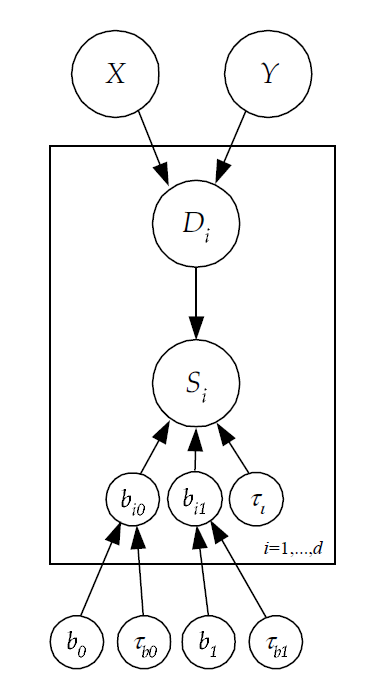
\includegraphics[width=0.3\textwidth]{Model_M2.png}
                    \caption{Model $M_2$ from \citet{madigan2005bayesian}.}
                \end{figure}
                
                \citet{madigan2005bayesian} instead utilised a graphical model to embody the relationship between position and RSSI (Figure \ref{fig:m2}). In their Bayesian Network, for each access point $i$ the distance $D_i$, transmit power $b_{i0}$, path loss rate $b_{i1}$ and noise $\tau_i$ are all conditionally dependant given the RSSI observed $S_i$. This signifies that given a set of these variables, the model can infer the most likely values for any connected values in the graph (for example, training data would give the X and Y co-ordinates and the signal strength, which can be used to infer all other variables given the graph's completely connected nature). Then during the on-line positioning phase, the user's most likely position is inferred from the AP variables established during the training phase and the observed RSSI values. Using this model they are able to estimate position assuming only the degradation of RSSI is roughly logarithmic and that all access points have similar behaviours ($b_0$ and $b_1$ are the global variables around which each specific access point's values are estimated). This method does require training data in order to calculate the maximum likelihood access point parameters, but with a very small number of training samples (around 20) and no other knowledge of the building they show that the model is able to estimate the user's location with a \textasciitilde50\% increase in median error compared to RADAR.
                
                While providing insights into the area under observation with little prior knowledge, these techniques are 'one-shot': a model is built from known values and then followed permanently thereafter. However, should the space be modified or new interference added at any point after the model is created, the solution would effectively need re-deploying to continue providing accurate estimates.
            
            \subsection{Adaptive Indoor Positioning Systems}
            \label{sec:adaptive}
            
                All of the previous techniques discussed have had two very distinct phases: off-line and on-line. During the off-line training phase, data is gathered with ground truths (guaranteed values such as user verified location) or models are calculated and then in the on-line positioning phase the observed RSSI values are used in the models to determine the user's most likely location. This section however will explore techniques that can improve gradually over time as more users traverse the space.
                
                Techniques covered to this point rely on electromagnetic waves and the detection thereof to paint a picture of the user's current location, however \citet{wang2012no} combined dead-reckoning (estimating relative location by tracking movement from a known point) and a broader range of sensors than most other techniques to estimate location. Traditional dead-reckoning is known to be relatively accurate at first, but random errors gradually accumulate and the estimation can become wildly inaccurate the further travelled from the starting point. This technique however relies on organically generated `landmarks' to help reset the accuracy of a user's current position as frequently as possible (Figure \ref{fig:dead}). These landmarks can range from elevators detected by accelerometer spikes to metallic areas detected by the magnetometer, each uniquely identified by the RSSI values surrounding the area. As the mean of the error generated by dead-reckoning is theoretically $0$, a landmark can be placed at the average location of all positions it has been identified at making exact positioning when the landmark is detected possible. While accurate to a reported 1.2m with no prior knowledge of the space and no deployment necessary, this positioning method must be permanently active from each landmark or the user will be unable to locate themselves. Also, even with techniques identified to only use the most effective landmarks this would still put a relatively heavy weight on the user's power supply through its always-on nature and the variety of sensors required compared to conventional RSSI measurement.
                
                \begin{figure}[h]
                    \label{fig:dead}
                    \centering
                    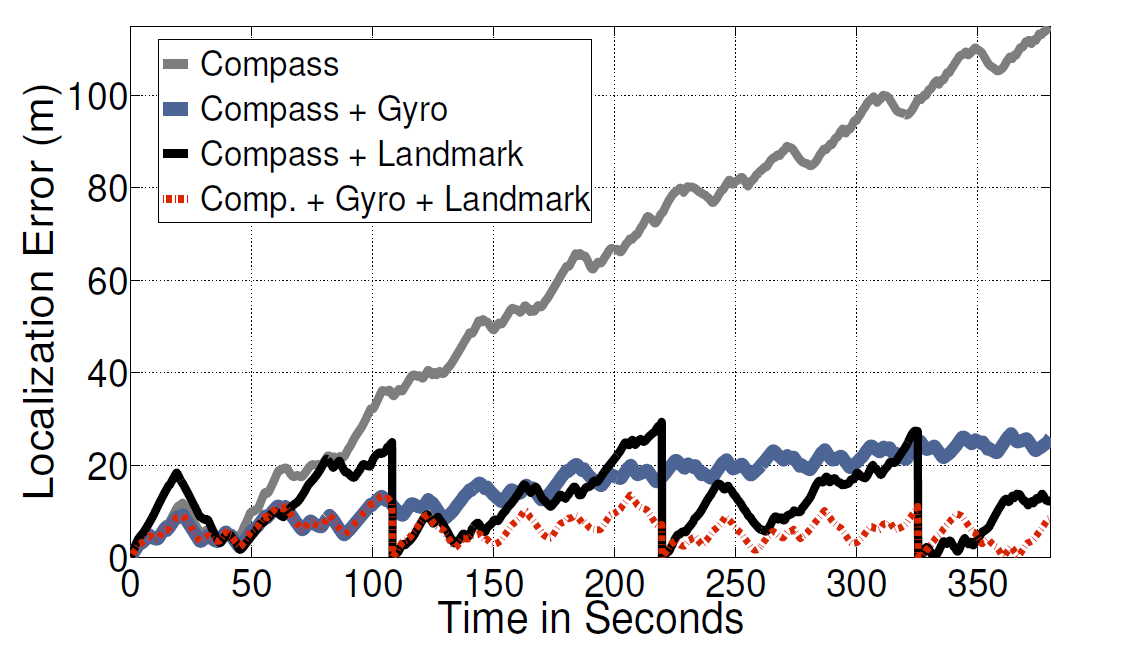
\includegraphics[width=0.7\textwidth]{dead.png}
                    \caption{Dead-reckoning accuracy found through experimentation by \citet{wang2012no}.}
                \end{figure}
                
                More conventional methods had also been gradually improved upon to provide sub-metre levels of accuracy by combining crowd-sourced data with probabilistic reasoning through a technique called `Horus' \citep{youssef2005horus}. The first step (and largest weakness) of the Horus system is the necessary collection of sample data from known locations to create an initial RSSI map. Data collected by users while positioning however now continues to feed back into the initial RSSI map as the team discovered that RSSI values from each AP are not independent with regards to time, so utilising an auto-correlation co-efficient ($\alpha$) helps to isolate useful measurements. This co-efficient defines how similar readings in an area have been and augments the expected distribution of RSSI values for that area to allow for a much larger range if all observations have been very similar.
                
                Using this modified RSSI map, positioning is then broken down into multiple steps; first the user's `discrete' area must be determined as the most likely position, given all of the access points that are currently visible (like a fingerprint). From here, the system uses a function of both the $N$ most likely locations weighted according to their normalised probabilities and the average signal strengths over a small time window to smooth out the estimate. Finally, the system enables tracking of small-scale variations by noting that a user's location cannot change more than their speed would allow. By this notion, if the user appears to have moved more than a threshold amount more than their previous movement, a small-scale error is assumed and so the system tries an estimation for all received AP RSSIs multiplied by $1$, $1+d$ and $1-d$ to find the highest likelihood and associated location.
                
                The final technique this paper will cover requires no prior knowledge of the space, extra deployments or a specific training set: Microsoft's `EZ' localisation system \citep{chintalapudi2010indoor}. The technique is centred around solving simultaneous equations to provide accurate estimates, similar to \citet{madigan2005bayesian} in looking for its parameters. However, the technique uses occasional measurements paired with GPS readings and clustering methods to reduce the search space to the most useful subset. 
                
                \begin{equation} \label{eq:EZdistance}
                    d_{ij} = 10^{\left(\frac{P_i - p_{ij}}{10\gamma_i}\right)}
                \end{equation}
                
                For each access point ($i$), the system attempts to solve for its X and Y location, transmit power ($P_i$) and path loss rate ($\gamma_i$). If the access point is visible from at least 5 locations where GPS lock was established ($j$), then these parameters can be uniquely identified through solving simultaneous equations (Equation \ref{eq:EZdistance}) for RSSI values ($p_{ij}$) from which the access point was seen and then using the gathered distances ($d_{ij}$) to trilaterate the 2D location of the AP. Solving even just one AP's parameters can cause a domino effect leading to more uniquely identifiable locations, solving more AP parameters and so on. Eventually though the dominoes stop and the system has to guess some parameters in order to continue and this search space can be incredibly large. To counter this, the EZ team created APSelect and LocSelect, two clustering algorithms that group access points and unknown locations into a single point if the observed RSSI values overlap by \textasciitilde90\%, thereby reducing the number of unknown variables the system has to solve for, taking only a minimal accuracy loss in the process.
                
                The space is then searched through to find a set of parameters with the minimum error using a combination of genetic searching and gradient descent. To start with, a set of solutions with completely random parameters are selected and their fitness (mean absolute error) evaluated. From here, the top 10\% are kept unmodified, 10\% are randomly re-generated, 60\% are made as a combination of 2 random parents from the last generation (and enhancing them through gradient descent) and the last 20\% are made by taking a single random solution from the last generation and tweaking each parameter by a random amount (from an exponential distribution to allow for occasional large changes). This combination of solution generation techniques avoids the large number of potential global minima that come with so many parameters while exploring the state space relatively quickly.
                
                One final optimisation applied to their method is accommodation for relative gain. By identifying proximate locations in which measurements were taken by two different devices, their average RSSI values can be compared to find their approximate relative gain difference and normalise their RSSI values for use in simultaneous equations. With all of these techniques combined, EZ was able to perform comparably to RADAR on larger scale deployments without all of the pre-deployment effort and the search for optimal parameters could be re-run as the space being localised changes and more data comes in. This technique benefits strongly from its adaptability and lack of required prior information about the space, but suffers minor drawbacks in the form of its marginally lower accuracy than techniques like Horus (Figure \ref{fig:EZHorusRADARComparison}) and the relatively high computational effort required to implement the technique and compute the results.
                
                \begin{figure}[h]
                    \label{fig:EZHorusRADARComparison}
                    \centering
                    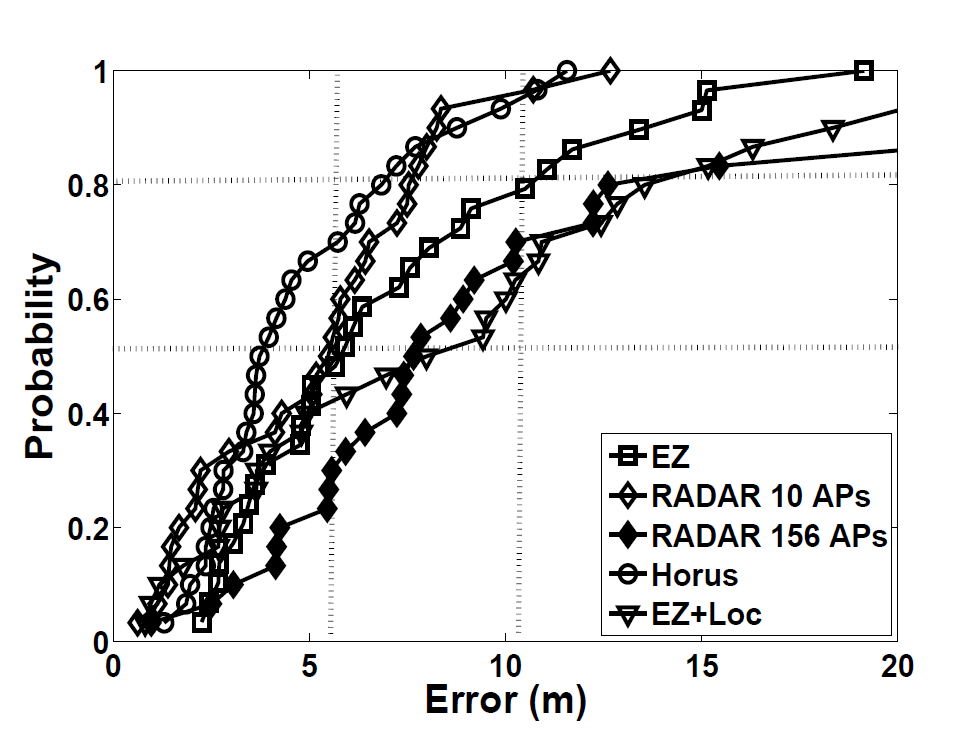
\includegraphics[width=0.7\textwidth]{EZHorusRADARComparison.png}
                    \caption{Cumulative distribution function of distance error comparing Horus, RADAR and EZ IPS techniques \citep{chintalapudi2010indoor}.}
                \end{figure}
                
                Following the rapid development of IPS techniques \citet{torres2014ujiindoorloc} identified the need for a definitive data set to compare them through and created the UJIIndoorLoc database. The data set comprises of a large number of user-verified co-ordinates and their respective RSSI values to every WLAN access point being monitored. As these measurements were carried out by a number of users (integrating height as a differentiating factor) with a number of devices this provides great ecological validity to the data set while still delivering reliable measurements. The validation set was also generated without guide markers, ensuring that data different from the training set was provided. With such a comprehensive data set it is then easy to emulate limiting factors of any data gathering technique, such as noise or poor coverage, and due to high demand the team also provided a map of the locations \citep{UJIIndoorLocMap}. However, data points extraneous to the buildings in question would have been useful to provide a complete picture of a user's day both inside and outside of the buildings.
            
        \section{Automated Floor Plans}
        \label{sec:floorplans}
        
            Floor plans of a building are often key to enabling detailed location-based analysis by providing boundary information and special characteristics of the space, but may not be available prior to a system's deployment. It is easy to see how a special purpose robot might use a combination of dead-reckoning and obstacle sensors to map a space using an exhaustive search, but the cost of the equipment and the size of the area being surveyed could easily render the technique infeasible.
            
            Other techniques for building floor plans rely on gathering a small amount of pre-requisite data and building upon the constraints that it gives. A technique for determining layout on a small (single floor house) scale is described by \citet{lu2012smart} for use on ``Smart Homes''. Smart homes are buildings with a notion towards autonomous control, such as turning on the lights in the hallway before the user physically enters the space, detected through a collection of sensors placed about the home. Here, it is required to have motion detectors placed on both sides of every door (to determine room connectedness), a magnetometer (to determine door orientation) attached to these pairs of motion detectors and light level sensors on every window (facing inside and out, to determine orientation through sunrise / sunset). While this is a very high deployment cost through the level of user involvement, the deployed sensors are then anticipated to be in continuous use as part of the smart home itself.
            
            By monitoring the sensors to see which sets fire simultaneously, they can then be clustered into rooms to determine how many doors and windows each room has, and which rooms they are connected to. With the room's interconnectedness established, the technique then minimises the space of potential arrangements using a set of simple heuristics (i.e. windows tend to be on external walls and buildings have as few corners as possible). Despite all of these restrictions, the technique was only able to minimise the set to 2 or 3 potential layouts from which a user must select. As this technique was designed to prevent having a user draw their own plan it satisfies its purpose, but does not provide a detailed enough picture for fine-grain analysis or larger areas of observation.
            
            A more general approach to generating floor plans based on a set of constraints however comes from \citet{charman1994constraint}. This method mathematically defines a set of rooms based on their rotation, reference point and dimensions and attempts to fit them into a given space by connecting their corners. As the rooms are placed, a set of constraints are then evaluated and back-tracked upon where necessary (e.g. Bedroom \#1 must be to the right of Bathroom \#2). By exhaustively generating solutions, the system is able to find all possible layouts of rooms, given the pieces of data / constraints supplied. While successful at producing floor plans for traditional housing layouts, the method could fall short with modern architecture that often contains complex shapes (not squares) and unidentified empty spaces.
            
        \section{Summary}
        \label{sec:relsum}
        
	        This chapter has now broken down the work surrounding building analysis into the data gathering, data localisation and floor plan generation steps and provided a variety of techniques that are applicable at each stage. When gathering data from users it has been shown that techniques exist to reduce the load placed on users and their devices, potentially increasing the amount of data that would be gathered in a crowd-sourced technique through more opted-in users. While users are of the utmost importance when performing any crowd-based operations, this report focuses mainly on applications of the data once collected.
            
            When localising gathered data, a theme has emerged centring around the use of RSSI to estimate distances from access points. Despite its complex nature, the  widespread use and coverage of wireless networks combined with the success of simple models make it an attractive choice for IPS. Techniques explored here covered the fundamentals of modelling radio signal propagation, then demonstrated more advanced and novel techniques inferring unknown parameters through machine learning for ease of deployment and increased accuracy alike.
            
            Finally sets of constraints were identified for generating possible floor plans based on estimated dimensions. While restrictive in their application to walls in the four cardinal directions, this fits common traditional layouts of buildings and it is anticipated that more complex arrangements could be broken down into rectangular subspaces to build in. Through combinations of the described techniques it can be envisaged that a building analytics framework could be built; this report however will now explore each individual component's potential and decide upon steps to be taken towards the framework's realisation.

    \chapter{Problem Analysis}
    \label{chap:problem}
    
        This chapter will explore the problem space involved with attaining the goals of the project. Primarily, this project is tasked with establishing a framework around which building analytic techniques might be developed or applied. This could include the development of any combination of the techniques covered in chapter \ref{chap:related} concerning crowd-sourcing the data, localising the data and modelling the space itself.
        
        Developing a complete system however would prove intangible for a project of this size as the system would require implementation across multiple platforms and likely multiple languages, carrying with it the interoperability complications and technical difficulties to navigate as opposed to research challenges. Furthermore spreading implementation time so thinly might also prevent any deeper evaluation as it would be hard to compare systems at such a high level. As such it would be wiser to focus on implementing a single component around which a system can be built.
        
        The first component to consider would be a modern crowd-sourcing tool-kit for specifying, gathering and collating some selection of data from sensors at minimal impact to the users. While implementing an application in Java using the techniques described in section \ref{sec:crowd} to enable gathering from a wide selection of Android devices would be beneficial to build from, it is known that a specific study into the factors surrounding crowd-sourcing data is running concurrently to this project \citep{IainBate}. Floor plan modelling using location data to feed a constraint solver such as that described by \citet{charman1994constraint} could also be an effective component. However, compiling such a complete set of data without implementing either of the previous components of the system would be very costly for such a small team, given the number of man hours it would take to exhaustively map out a significant area. Therefore, the most useful component to create as part of this project would be an Indoor Positioning System around which other techniques may be developed. As demonstrated by \citet{torres2014ujiindoorloc}, there exists a high demand for open implementations of such components and thanks to the existence of such sample data sets, the costs of testing and comparing such techniques are greatly reduced.
        
        As explored in section \ref{sec:ips}, there exist a multitude of techniques for localising users in an indoor space with varying degrees of accuracy. The goals of this project however, limit the range of applicable techniques as the model should be created from readily available sources of information. While this immediately rules out any infrastructured techniques as the installation of extra equipment severely limits the domain space that can be modelled, this project will also avoid those that require a large set of ground-truth, domain-wide test data as they are again limited in their application. With these restrictions in place the most interesting systems to study would be: RADAR \citep{bahl2000radar}, landmarked dead-reckoning \citep{wang2012no} and EZ \citep{chintalapudi2010indoor} from those evaluated in chapter \ref{chap:related}.
        
        RADAR provides one of the highest levels of accuracy of all reviewed techniques for relatively low localisation and model-building cost as it is based around a pre-existing floor plan. Using this floor plan, the technique estimates the RSSI of every AP by using a simple formula modelling the signal's attenuation through walls and across space. In situations where detailed floor plans are already available, using this method could be the most efficient means for determining building usage metrics as the model building process is skipped entirely and user positions can be determined immediately. However, floor plans are not always complete, universally accessible nor consistent with flexible spaces such as exhibition centres. Because of this limitation in combination with the lack of information generated by skipping the modelling process, this technique is not useful for the project.
        
        Landmarked dead-reckoning appears to rectify most of these concerns as the technique requires no previous knowledge of the space (by dead-reckoning from a known point) and creates its map of landmarks that are potentially much less dependent on the flexible properties of the space (such as elevators and stairs). This enables the modelled space to change over time while preserving a relatively high level of relative location accuracy. Therein however lies the problem with using this technique to measure space utilisation as it can only detect relative movement as opposed to independent single-point localisation. This is not to say that the technique would be difficult to gather sample data as \citet{torres2015ujiindoorlocmag} provides the full complement of magnetometer, accelerometer and (in conjunction with future data to be provided by \citet{JoaquinEmail}) RSSI readings necessary to implement such a system. The worry is more about the load placed on prospective user's devices and how to gather meaningful results without the storage requirements becoming infeasible. As shown in the UJIIndoorLoc-Mag database, the \textasciitilde40,000 data points only correspond to \textasciitilde300 short relative motion traces so it is not unimaginable for the data sets to quickly get out of hand, especially if a user were to store multiple day's worth of data before a storage opportunity arises. Solutions to these problems could involve modifying the sampling frequency to reduce the load on the user's device and the amount of data held for analysis, but it is unknown as to how this would affect the accuracy of the model due to the precise nature of the landmarks. Also, the test data and initial research do not cover the prospect of spending a large period of time walking around the same space with no significant landmarks. In these cases, the behaviour would return to basic dead-reckoning and continually stack up inaccuracies, potentially invalidating the data. For these issues in combination, landmarked dead-reckoning does not significantly work in the project's favour.
        
        EZ however, implements a system requiring a very simple set of independent client-side measurements backed up by a server-side model that can adapt to a changing space as the set of observations grows, without human intervention (such as specifying a new floor-plan like RADAR). With this technique, RSSI measurements are provided along with GPS co-ordinates (where possible) to estimate the relative location and signal transmission properties of the access points being observed. This simplicity of the data required to build the model along with that of the model itself also makes it useful for research into building analytics as it reduces the effort required to crowd-source the data in the first place and reduces the complexity of any floor plan model wishing to reinterpret the EZ data.
        
        Assuming that the crowd-sourcing programme or test data input provides a reading of all RSSIs available (as already required by a wide range of infrastructureless indoor positioning systems) alongside the occasional GPS location, EZ will be able to provide a model for localising those without position data and any future measurements made. Furthermore, assuming that the floor plan modelling technique is also able to make use of the positioning data, the output of running EZ on the original data set will still be useful regardless of the technique's ability to interpret the generated AP parameters to some degree. Combining these assumptions with a large set of sample data such as that provided by \citet{torres2014ujiindoorloc}, the EZ localisation component can then be developed independently of any crowd-sourcing or floor-plan modelling strategies that may follow as the initial component of the proposed building analytics framework.
        
        Unfortunately, \citeauthor{chintalapudi2010indoor}'s implementation of EZ is proprietary property of Microsoft and as such was not available for inclusion in this project. Re-implementing the system however provides an opportunity to evaluate the specification provided against a number of non-functional metrics as well as the modelling accuracy. For example, re-implementation and testing against a new data set may highlight a number of hidden assumptions and scenarios in which the model is flawed impacting directly on its applications for the real world and the ease of development for a more novice team. This project's implementation will also be aligned with a different set of goals, such as extensibility and flexibility (with regards to testing parameters and components) as opposed to the raw throughput for a single space that a commercial solution might strive for.
        
        In summary, this project so far has provided a number techniques for each potential component to be made as part of the building analytics framework. Having reviewed the options available, this project will now create an EZ-style IPS component as the technique appears to be the most in line with the project's desired use case. Following that it will evaluate the reference implementation (aiming to be made freely available upon the project's completion) against the UJIIndoorLoc data set to achieve a number of the project goals established in chapter \ref{chap:intro}.
 
	\chapter{Method}
    \label{chap:method}
	
		This chapter will cover the development of an indoor positioning system from which location data and Wireless AP models can be extracted for use as part of a general building model. The model will follow the techniques as specified in the EZ localisation system \citep{chintalapudi2010indoor} with measurements from the UJIIndoorLoc data set for testing and evaluation purposes \citep{torres2014ujiindoorloc}. This chapter will also identify some weaknesses in the specification of EZ and propose the Heuristic-EZ localisation system to compensate.
		
		\section{System Specification}
        \label{sec:sysspec}
            
            Microsoft's proprietary implementation of EZ by \citeauthor{chintalapudi2010indoor} consisted of ``about 7000 lines of C\# and Python code'' encompassing all of the client-server communications, data gathering and off-line modelling / on-line localisation operations. By separating out the data processing elements of EZ from the rest of the system, this implementation of EZ can take advantage of languages with more powerful built-in mathematical functionality without worrying about handling sensors and external communications. As such this project will pursue an implementation in Matlab 2015b consuming a .CSV file of pre-gathered measurements and outputting two .CSV files containing all localised points and the AP parameters separately. This allows future efforts into crowd-sourcing to take advantage of techniques available to other languages while still piping data into this implementation of EZ. It will also allow floor plan modellers to be selective as to which types of data they wish to use to generate their models, again in their language and platform of choice.
            
            \begin{figure}[h]
            \label{fig:EZControl}
            \centering
            \resizebox {\textwidth} {!} {
            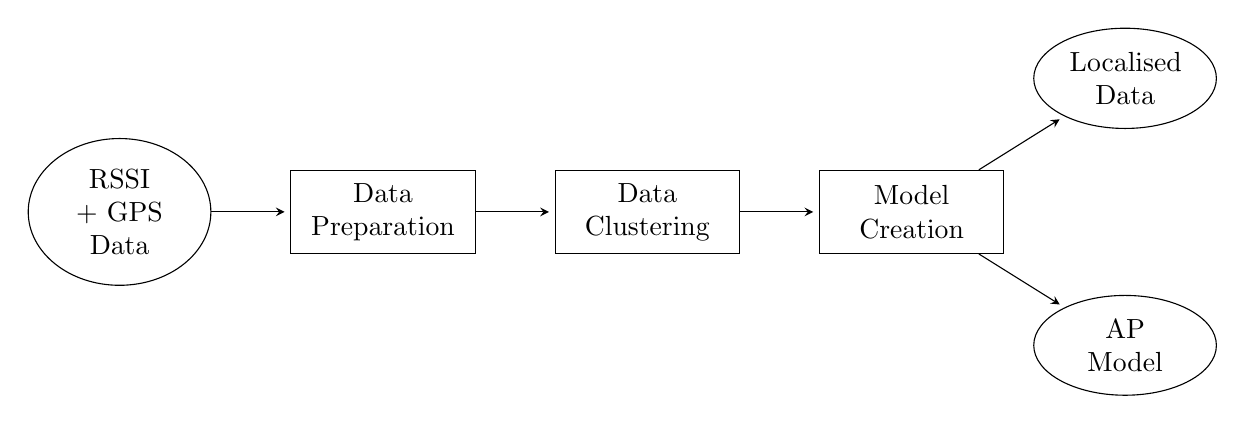
\begin{tikzpicture}[%
            ->,
            shorten >=2pt,
            >=stealth,
            node distance=1cm,
            process/.style={%
            	rectangle,
            	text width=6em,
            	minimum height=3em,
            	align=center,
            	draw
            },
            data/.style={%
            	ellipse,
            	text width=4em,
            	align=center,
            	minimum height=3em,
            	draw
            }
            ]
            \node[data] (1)                                 {RSSI + GPS Data};
            \node[process] (2) [right=of 1]                 {Data Preparation};
            \node[process] (3) [right=of 2] 				{Data Clustering};
            \node[process] (4) [right=of 3]                 {Model Creation};
            \node[data] (5) [above right=of 4]              {Localised Data};
            \node[data] (6) [below right=of 4]              {AP Model};
            
            \path (1) edge             node {} (2)
            (2) edge                   node {} (3)
            (3) edge                   node {} (4)
            (4) edge                   node {} (5)
            (4) edge                   node {} (6);
            \end{tikzpicture}
	        }
            \caption{EZ Control Flow}
	        \end{figure}
            
            EZ's specification then breaks the system down into a set of components, each of which is able to operate independently of the others or chained together for various effects. To this end, the project's implementation of EZ will take a pipe \& filter approach, allowing each component to affect the data in turn before passing it on to the next (see Figure \ref{fig:EZControl}). These components will all operate without knowledge of the other's actions and upon the same data format, such that components may be changed for different versions or removed entirely without significantly impacting the program's flow.
            
            The creation of EZ's model is the first and only mandatory component specified, but also comes as the final piece of any system variant that might be created. Given a set of data this component will attempt to create a model based on the idea that with enough already localised measurements of RSSI from an AP, some basic parameters can be estimated about that AP (giving the AP model data). Then if a measurement without GPS data can view enough parameterised APs, then its location can be trilaterated using simultaneous equations (this will be covered in detail in section \ref{sec:modelcreation}).
            
            However, as is also specified, the data can be effectively refined and reduced before it is passed to the model creator through preparation and selection of the most useful pieces of data. The most prominent piece described for preparing data is that of gain estimation as \citeauthor{chintalapudi2010indoor} report finding gain differences of up to \textasciitilde14dB across devices. This could significantly distort models generated using that data by making measurements taken at the same location on different devices appear very different by RSSI. To alleviate some of these problems, they proposed the Relative Gain Estimation Algorithm (RGEA) which looks for small, consistent differences in RSSI measurements and creates a set of estimated differences in gain across devices. By solving these differences as a set of simultaneous equations, the gain values of each individual device can then be estimated and used to correct the input data (covered in full in section \ref{sec:dataprep}).
            
            Finally covered is the selection of specific data points to use when modelling through the use of hierarchical clustering. This clustering algorithm aims to group data points of 90\% or greater similarity and then nominate a representative from each group to be passed to the model. The algorithm is run twice on the same data set, but once to select the most useful Access Points (APSelect) and once to select the most useful measurement locations (LocSelect) for different reasons. APSelect is run to reduce the number of APs modelled as the team observed up to ``160 APs across a single office floor'', potentially leading to an over-constrained model and excessive modelling time. LocSelect however, is necessary to prevent biases in the model where too many measurements from the same location may reduce accuracy in others.
            
            The ordering of these components is of course fixed as clustering data without correcting for gain could miss potential groupings and correcting the gain of already localised points would lead to inaccuracies. The components can however be avoided entirely (except for modelling) as \citeauthor{chintalapudi2010indoor} experimented with. This project will make comparisons of its implementation to their claims using their `\emph{LARGE}' data set as its size is more comparable to a single floor of a building in that of the work by \citet{torres2014ujiindoorloc}.
		
		\section{Data Preparation}
        \label{sec:dataprep}
        
            In order to compensate for artificial noise created by differences in gain across devices measuring RSSI at the same location, the RGEA estimates these differences and applies them to the data set. However, with only a subset of the data having a known location, the RGEA has to use RSSI to guess at `proximate' locations. The specification states that measurements are deemed proximate if the average difference between RSSIs is less than 3dB. For each pair of devices ($k_1,k_2$), these pairs of measurements are then gathered into a set $M^{k_1k_2}$ and compared to get the average difference (Equation \ref{eq:avggaindiff}). This relative gain is then plugged into equation \ref{eq:stddevgain} to calculate the standard deviation of that relative gain from the difference in all comparable measurements.
            
            \begin{equation}
            \label{eq:avggaindiff}
                \Delta G^{k_1k_2}=\dfrac{1}{|M^{k_1k_2}|} \sum_{(p_1,p_2)\in M^{k_1k_2}} (p_1 - p_2)
            \end{equation}
            
            \begin{equation}
            \label{eq:stddevgain}
                \sigma(\Delta G^{k_1k_2})=\dfrac{1}{|M^{k_1k_2}|} \sqrt{\sum_{(p_1,p_2)\in M^{k_1k_2}} (p_1 - p_2 - \Delta G^{k_1k_2})^2}
            \end{equation}
            
            Because these relative gains are transitive (i.e. $\Delta G^{k_1k_3} = \Delta G^{k_1k_2} + \Delta G^{k_2k_3}$), any pairs of devices with proximate locations can then be chained together with other device pairs to create a system of simultaneous equations. Finally a random device as part of this system is selected and chosen to have some value of gain and so the system can be solved. As this is an estimate however, the equations are weighted according to their standard deviation or in effect their likelihood of being accurate.
           
            Implementing this short specification however, leads to incorrect results. The main discrepancy is the selection of RSSI readings to include when comparing a pair of measurements. For completeness, the UJIIndoorLoc data set includes every invisible AP as a measurement of 100dB to mark it as an invalid measurement. If all readings (including invisible markers) are compared for a pair of measurements, then in spaces where only a small proportion of APs are visible at any given location, all locations will be deemed proximate as all invisible APs register a difference of $0$. The opposite however also causes problems, if only points visible at both locations are compared, then being equidistant from a single AP could cause the whole measurement to be deemed proximate (see Figure \ref{fig:overlap}). The solution is to compare all readings visible in either measurement, such that if the measurement were to be localised using that set of points, they should be equal. However, including readings in this manner with the UJIIndoorLoc positive invisibility indicator causes any single difference in AP visibility, no matter how weak (i.e. -99dB), to be marked as not proximate in error. The simple fix was to change all 100dB readings to -100dB.
            
            \begin{figure}[h]
            	\centering
            	\begin{minipage}{0.45\textwidth}
            		\centering
                    \label{fig:overlap}
            		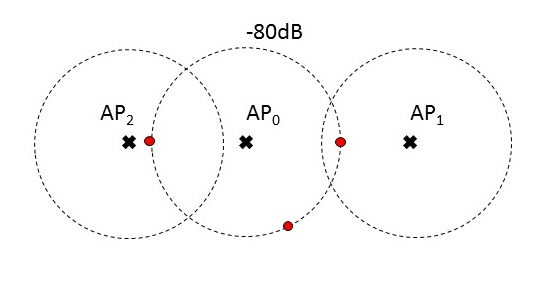
\includegraphics[width=\textwidth]{single_overlap.jpg}
            		\caption{All locations demonstrated would be marked as proximate with $0$dB gain when only using APs visible at both locations.}
            	\end{minipage}\hfill
            	\begin{minipage}{0.45\textwidth}
            		\centering
                    \label{fig:wall}
            		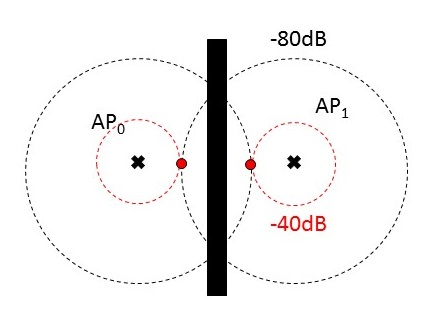
\includegraphics[width=1\textwidth]{wall.jpg}
            		\caption{Across wall case mistakenly marked as proximate with $0$dB gain.}
            	\end{minipage}
            \end{figure}
            
            With the specification implementation producing feasible results, it was at this point that the technique was to be validated against some known values. With no provided gain values for the devices in use by UJIIndoorLoc however, it was necessary to attempt to calculate them separately. To this end another relative gain estimator was created using the ground truth location values to specify exactly which pairs of measurements were proximate. The first major change was the addition of a general location translator to the data preparation phase as measurements were gathered within a few hundred metres of each other, but the latitude values started at \textasciitilde4,865,000m. The other major difference was a factor of speed. As the location comparison only needed to compare the difference between latitude and longitude as opposed to the average difference of up to 520 APs, the ground truth calculator performed over 2 orders of magnitude faster!
            
            Through experimentation and comparing the RGEA's output with the newly calculated values, several other faults in the implementation came to light. The first was that when calculating the average difference between measurements for inclusion in the set $M^{k_1k_2}$, it was meant to be the average \emph{absolute} difference being less than 3dB. Errors in light of this fault arose with measurements where readings balanced out with positive and negative differences (such as being opposite sides of a wall). For example the average difference of (-20dB, 20dB) for 2 APs is $0$dB, causing the points to be falsely identified as proximate with no relative gain (see Figure 4.3).
            
            Despite removing the majority of the falsely proximate points through this fault, the technique would still produce a very small number proximate points for those that should have none in common due to random fluctuations in the RSSI. Because of the transitive nature of the relative gain, this lead the algorithm to attempt to include erroneous relationships in its system of simultaneous equations, rendering them either unsatisfiable or wildly overestimating the gain applied to certain devices. As such the simplest solution was to impose a minimum number of proximate points for a relative gain to be of great enough significance to consider in the system.
            
            Given the computational and general modelling complexity of EZ's RGEA, it was theorised that there could be some simpler proximity metric with computation times more similar to those of the ground truth estimator. This lead to the creation of the first simplified component of this study: 'Heuristic RGEA'. Rather than essentially re-calculating the potential relative gain for every point, this technique compares the AP visibility of the strongest RSSIs at each location. Simply put, for each pair of measurements, if both samples have at least a certain number of RSSIs above some strength threshold, the locations can be deemed proximate if the set of strongest RSSIs is similar \emph{by AP ID alone}.
            
            This metric should prove effective because of the abundance of APs shown in both \citeauthor{chintalapudi2010indoor}'s study \citep{chintalapudi2010indoor} and the UJIIndoorLoc data set \citep{torres2014ujiindoorloc} creating an AP fingerprint for most locations. Initial tests however did highlight that the ordering by strength within these fingerprint sets is almost never identical due to random fluctuations in RSSI, leading to an extremely pessimistic judgement of proximity. As such the final implementation only specifies a minimum overlap between the two. With a number of parameters available to tune that may greatly affect the outcome of relative gain estimation (including the average difference threshold for EZ's RGEA and the size of the strongest set to compare in Heuristic RGEA), both techniques will be experimented with in section \ref{sec:rgeaeval}.
		
		\section{Hierarchical Clustering}
        \label{sec:datacluster}
        
	        In EZ, hierarchical clustering is used to effectively reduce the set of data fed into the modelling process both for speed and to reduce bias. The technique is used both as part of processes called APSelect to determine which APs are to be modelled by the system and LocSelect to choose the subset of all measurements around which to model them. To prepare the data for clustering, each measurement is normalised across the range ($0 \rightarrow 1$) for RSSIs ($-100 \rightarrow 0$) where any unseen APs have their RSSI set to -100dB. Clusters are then grouped if the average absolute difference between every pair of measurements across clusters is less than $0.1$ (>90\% similarity). Finally the point elected to represent each cluster is that which is most constrained (i.e. can see the highest number of GPS localised measurements in APSelect or just a binary indicator of being GPS locked in LocSelect) or the most similar to the rest of the cluster in the case of ties.
	        
	        Interestingly, \citet{chintalapudi2010indoor} only discuss the effect of removing fringe-case data points for speed improvements with regards to the modelling stage. However, there may exist more significant measurements or (less commonly) APs in very close proximity which should also be clustered into a single representative point. This has the effect of reducing bias towards these locations by removing the error incurred from their use in the modelling stage.
	        
	        While simple and theoretically sound, this naive implementation of clustering doesn't take into account the potentially sparse nature of the input data with regards to AP visibility. When run for APSelect over the UJIIndoorLoc data set, more than 10,000,000 full data set comparisons were required (taking hours to complete alone without modelling) and LocSelect over a thousand point data set was rendered computationally intractable. The results also suffered a similar problem to that of the RGEA where given enough measurements / APs, `invisible' RSSIs outweigh those of any significance, so the clustering is detrimentally aggressive.
	        
	        In an attempt to minimise these issues, MATLAB's sparse matrices can be employed if making full comparisons per point (to little effect) but to get a less aggressive clustering, techniques explored during the creation of the RGEA can be employed. The first of these is to use a much simpler indicator as to whether the points might be similar before running the calculation, the most obvious of which is simply the set of non-zero measurements. If the set overlaps enough (differing in size dependent on the number of non-zero measurements per point) then a comparison over the union of both of these sets should be run.
	        
	        This idea is then extended to only consider the high strength measurements from each point as they are the least prone to noise and likely to be reliable for modelling. By only considering measurements above a threshold this comparator also introduces a 'zero' category where measurements from certain points were not considered reliable enough and skipped entirely, providing a significant speed increase by immediately removing them from clustering. Removing these fringe-case measurements however, may also impact on a location's instant recognisability. For example, if an AP belongs to a neighbouring building and is only visible in a very small area on the edge of the building being modelled, then seeing that AP could immediately narrow down the location of the data point (see Figure \ref{fig:fringe}). The impact of these various attempts at data set reduction will be evaluated in section \ref{sec:modeleval}.
		
		\section{Model Creation}
        \label{sec:modelcreation}
        
            This final section will cover the main modelling component of the system, taking in processed data from the previous components and deriving a model of the AP layout and signal transmission properties surrounding them. Interesting challenges of dealing with real-world scenarios (discovered through rudimentary verification testing) will be explored and the process of using the model to localise measurements will be described.
        
            \subsection{Off-line Learning}
            
                The off-line learning phase of this component is concerned with translating the input data into a simple model of all APs through solving systems of simultaneous equations. For each AP, the system has to choose a distance to each observation $d_{ij}$ (and by extension a latitude and longitude location), transmission power $P_i$ (starting strength) and path loss rate $\gamma_i$ (signal strength fall-off curve). If the model were perfect, these 4 parameters could be uniquely determined (a single global minimum error) from just 5 observations of the AP from known locations by minimising the RSSI error produced by the fitness function shown in equation \ref{eq:modelerror}.
                
                \begin{equation}
                \label{eq:modelerror}
                    error_i = \frac{1}{N}\sum_{ij}|p_{ij} - P_i + 10*\gamma_i\log{d_{ij}}|
                \end{equation}
                
                This model however lacks the ability to show sudden drops in signal strength and instead will choose to model the AP as closer to its observations with a higher path loss rate (as demonstrated in their study \citep{chintalapudi2010indoor}). As the solution space per AP is so large, this inaccuracy coupled with the potential random fluctuations in RSSI can lead to a large number of plausible parameters. \citeauthor{chintalapudi2010indoor}'s implementation employed a complex genetic algorithm considering many solutions per iteration in order to explore the space quickly. For drastically reduced implementation and modelling time however, this project opts to use a constrained version of Matlab's simulated annealing.
                
                The search space is constructed with reasonable allowances for signal transmission parameters (according to \citet{chintalapudi2010indoor}) and a bounded space around the included observations. Within that, the starting point is set as the average location of the included observations as might be common in a central AP deployment. This starting point is of lesser significance however, as simulated annealing provides a non-deterministic element to the gradient descent unlike other function minimisers, leading to less reliance on a good starting point. The main constraint on the simulated annealer is actually over the sufficiency of its output; given its semi-random, single solution nature, it is possible for the annealer to miss all plausible solutions and output a model-skewing set of bad AP parameters. As such, if the annealer's solution re-localises the modelling data to a median error of more than 10m, it is re-run up to a maximum of 10 times at which point the AP is deemed unsatisfiable and removed from the model.
                
                After attempting to model several APs it became apparent that a much larger proportion was being deemed unsatisfiable than initially anticipated, despite having a significant number of observations. The problem with these APs was that they appeared to be located on other floors of the same building. While theoretically plausible given enough data and time to model the extra dimension for AP placement, this project aimed to remain in the more proven 2D subspace (as demonstrated through the review of work in section \ref{sec:ips}). As such, the set of weak measurements coming through the floor to a small area was being interpreted as a large distance from the AP, but then being modelled laterally rather than vertically (see Figure 4.5).
                
                \begin{figure}[h]
                	\centering
                	\begin{minipage}{0.45\textwidth}
                		\centering
                        \label{fig:fringe}
                		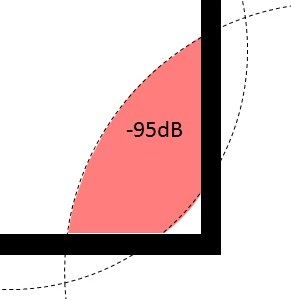
\includegraphics[width=0.7\textwidth]{fringe.jpg}
                		\caption{Red area marking the localisable fringe-case zone of a building.}
                	\end{minipage}\hfill
                	\begin{minipage}{0.45\textwidth}
                		\centering
                        \label{fig:vertical}
                		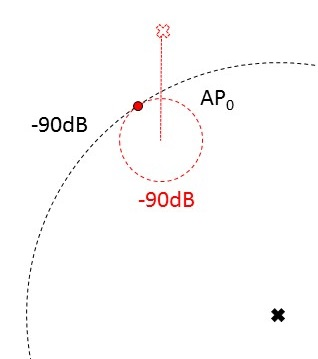
\includegraphics[width=0.7\textwidth]{vertical.jpg}
                		\caption{Visual representation of the difference between modelling an AP vertically (red) and laterally (black).}
                	\end{minipage}
                \end{figure}
                
                While potentially very useful towards localising to a very specific area of a floor, such a small area of coverage would be impossible to model without greatly expanding the search space for every AP. Given that these signals were also passing through concrete, electrical cables and various pipes to be received, the signals might also be particularly prone to interference and as such inaccurate beyond identifying the general area that the measurement was taken. Without ground truth data about the APs that would allow for model comparison and preparatory pruning of those less directly useful APs (though more thorough data covering alternative spaces are anticipated through communication with \citet{JoaquinEmail}), a thresholding heuristic was devised in place.
                
                Thresholding simply prunes all RSSIs below a certain level for both modelling and localisation purposes in an attempt to split the 3D space into an independent set of 2D subspaces. Pruning in this manner will significantly reduce the localisable area surrounding an AP, but as a consequence it should also increase the overall reliability of the set of measurements used by reducing the signal-to-noise ratio. However, it is also necessary to prune the same measurements for localisation so as not to incorrectly extrapolate the path loss rate at longer ranges, further reducing the localisability of most points.
                
                This technique could also be applied as an alternative to the hierarchical clustering component by simply requiring APs and measurements to have a minimum number of high strength RSSIs. While it is anticipated that this would not cluster extremely similar, high-strength points as discussed in section \ref{sec:datacluster}, it should be able to identify weak, fringe-case points in just linear time. By using some form of parameter optimisation (i.e. simulated annealing) over a combination of these thresholding techniques, it was anticipated that a strong separation across floors could be established without over-restricting the coverage of each AP. This level of complexity however would run contrary to the initial time savings made and potentially over-fit to each set of data. As such, experiments will be performed in section \ref{sec:modeleval} to determine a general purpose set of parameters that increase localisation accuracy without drastically restricting coverage.
                
                The final parts of the modelling process deal with insufficiencies in the input data: AP propagation and the ERSGA. AP propagation tackles the fact that GPS or other positional data is often not available throughout buildings and as such not all modelling data will have pre-associated positions. The solution is to iteratively generate AP parameters based on the localised data points and then localise new data points using the parametrised APs. The EZ Random Solution Generation Algorithm (ERSGA) however attempts to create AP parameters where there are simply not enough points observing it. While novel and potentially effective at producing models for areas poorly covered by the data with a full genetic algorithm, for this project it would add needless complexity (both for implementation and at run-time) to increase accuracy in the fringe-case areas that most components so far have sought to eliminate. As such the ERSGA is not implemented in this project and the assumption is made that a crowd-sourced data set should be suitably thorough and cover all useful locations.
            
            \subsection{On-line Localisation}
            
	            Localisation of new data points using this model is a much simpler process, simply plugging in the observed RSSIs for all modelled APs into equation \ref{eq:EZdistance} to obtain an estimation of distance. As these APs also have a fixed location, so long as the data point can see at least 3 modelled APs the location of the data point can be found through trilateration. Even with the inaccuracies produced by random fluctuations in RSSIs, there should exist a single global minimum for distance error when solving for the latitude / longitude location. This combined with the fact that the solution only requires the two location parameters, it is just as effective and much faster to use a least-squared error simultaneous equation solver rather than including the overheads associated with a simulated annealer.
	            
	            It is unexplored at this point however as to how the selection of modelled APs from which the point is localised might affect accuracy. For example, during the AP propagation phase of modelling, a data point is localised as soon as enough of its observed APs are parametrised but it might be more effective to restrict localisation to more reliable measurements. To this end, using the thresholding technique from the modelling phase will impose this restriction, but the maximal set heuristic from other components can also be applied in a similar manner. By restricting localisation to calculate over the strongest (and most likely reliable) RSSIs, the system might be able to achieve higher localisation accuracy by avoiding weaker conflicting measurements where possible without removing coverage outright that might occur from thresholding. As such the various combinations of restrictions, component types and localisation methods will be evaluated for accuracy in section \ref{sec:modeleval}.
	            
		\section{Summary}
		
			This chapter has described the process of creating an EZ-style IPS and the various tweaks required to make it more feasible in a larger real-world deployment. The original specification supplied by \citet{chintalapudi2010indoor} was broken down into a number of components through which the data could be pre-processed for reduced modelling time / increased localisation accuracy and explored independently. In every case, the specifications of the pre-processing components were found to be inaccurate, invalid in edge cases or simply not scalable to the size of the data set under test. Fixes for these issues were identified, implemented and then extended to other components where it could theoretically improve the overall modelling time or accuracy.
            
            These modifications focused around simple changes that might remove less reliable or edge-case data points, namely through use of the maximum strength RSSIs per data point or removing any values below a certain threshold. While it was noted that these edge-cases could be used to easily identify very specific regions of the space being modelled, there currently exists no mechanism in this set of techniques to isolate and represent them. Finally, the application of those modifications to the modelling and localisation component was investigated, along with a reduction of the EZ specified genetic algorithm to a simulated annealer for significantly reduced implementation, run-time and evaluation complexity. Throughout this process a number of generic parameters were discussed; this in combination with the number of interchangeable components makes the upcoming experimental analysis a must in order to identify the most significant changes and combinations available (a copy of the software developed here is made available on GitHub \citep{git}).
        
	\chapter{Evaluation}
    \label{chap:eval}
    
        This chapter will identify objective measures of success from the outputs of each of the components discussed in chapter \ref{chap:method} and provide surrounding commentary. This process will require the design and implementation of a number of experiments running both individual components and combinations thereof over the aforementioned UJIIndoorLoc data set \cite{torres2014ujiindoorloc} to evaluate the system and techniques as a whole. Results gathered will aim to reflect the general purpose performance of the algorithms for their application in other systems and provide a comparable metric to those produced by \citet{chintalapudi2010indoor} for verification. Where possible, recommendations of parameters for general-case performance will be made and short-comings of the data set itself will be highlighted to assess the expected real-world performance of the system.
    
	    \section{Relative Gain Estimation}
	    \label{sec:rgeaeval}
        
            The first component to be evaluated is the relative gain estimation algorithm as the accuracy of its results may have a strong impact on all subsequent components. This section will assess the RGEA's feasibility both as a general purpose proximity test and for relative gain estimation, and provide a recommended set of parameters for future use. Both the EZ and heuristic implementation of the RGEA have a small number of configurable parameters, but given their continuous nature, an exhaustive search for a `best' combination would be intractable and likely fit specifically to this data set. To avoid this, a selection of values for each parameter across the most likely useful input range have been selected such that the tests are representative without becoming overwhelming (see figure \ref{fig:rgeaparams}).
            
            \begin{sloppypar}
            As described in section \ref{sec:dataprep}, the parameters surrounding EZ's testing will be the average RSSI difference threshold below which the location is deemed proximate (\texttt{prox\_threshold}) and the minimum number of common APs observed between points (\texttt{min\_AP\_overlap}) before they are considered for calculation. The Heuristic method however will look for relative improvement with respect to the minimum strength of RSSIs to be considered (\texttt{min\_AP\_strength}), the size of the set of high strength measurements (\texttt{num\_strong\_APs}) and the required overlap across these sets for the points to be marked as proximate (\texttt{min\_strong\_overlap}).
            \end{sloppypar}
            
            \begin{figure}
                \label{fig:rgeaparams}
                \centering
                \begin{tabular}[h]{| c | c |}
                    \hline
                    Parameter & Range \\ \hline
                    \texttt{prox\_threshold} (dB) & $2, 3, 4, 5, 7, 10$ \\
                    \texttt{min\_AP\_overlap} & $1, 2, 3, 4, 5$ \\ \hline
                    \texttt{min\_AP\_strength} (dB) & $-100, -90, -80, -70$ \\
                    \texttt{num\_strong\_APs} & $2, 3, 4, 5, 7, 10$ \\
                    \texttt{min\_strong\_overlap} & $2, 3, 4, 5, 6$ \\ \hline
                \end{tabular}
                \caption{Experimental parameter ranges for RGEA evaluation}
            \end{figure}
            
            The experiments run will compare both techniques' ability to identify relative gains against the values provided by the ground truth estimator run over the same data set as no actual values were provided for individual devices. It is important to note that only relative gains can be compared rather than the output absolute values as a relative gain of +7dB between two devices could be interpreted as +7dB gain on one device or -7dB on the other, leading to a potential double of the error being reported for a correct gain calculation. First however, experiments will be run to see how efficiently each technique identifies proximate locations as a means of testing the validity of the theory surrounding them.

		    \subsection{Proximity Determination}
            \label{sec:prox_est}
            
                This experiment will run the proximity determination sub-components of each RGEA type against one another to report on their efficiency. This will be determined not only from the percentage of proximate pairs available that are correctly defined as such, but also the ratio of correctly identified proximate pairs to falsely identified proximate pairs. These results should provide insight as to how useful the algorithm will be in practice as not many proximate pairs in general would demonstrate a pessimistic approach with little benefit to running the algorithm but a low chance of accidentally making it worse as well. An overly optimistic result with a large proportion of falsely proximate pairs however might do more harm than good on its inclusion by mangling the input data with non-existent gain differences.
                
                The selection of points deemed as proximate will be determined using the ground truth estimator that marks all pairs of measurements (across devices) within 1 meter of each other on the same floor. The input data for this first round of tests will use the entire UJIIndoorLoc data set, including all floors and buildings. The data will not be pre-processed in any way and only the ground truth estimator will be able to make use of the locations assigned to each point. It was theorised that use of the entire data set would be useful even when only modelling a 2D subspace as the gain applied to each device should be consistent, no matter the location. Identifying as many of the relative gain differences as possible would hopefully then reduce the artificial noise applied even in spaces where no proximate points exist. 
                
                The assumption was that inclusion of other floors and buildings in a single pass shouldn't adversely affect the result (other than drastically increasing the run-time) as the RSSI gap / AP fingerprint between each floor and building should be significant enough such that no points across floors are marked as proximate. The pre-processing elements of this system are also deterministic unlike the modelling element, so each run should yield the same results.
                
                \begin{figure}[h]
                	\label{fig:ez_overlap_prox}
                	\centering
                	\begin{minipage}{0.5\textwidth}
                		\centering
                		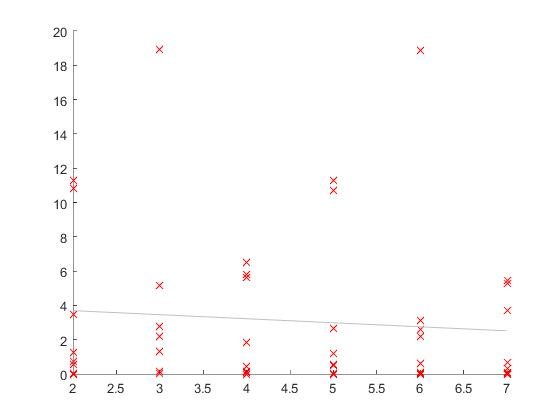
\includegraphics[width=1\textwidth]{ez_overlap_prox_correct.jpg}
                	\end{minipage}\hfill
                	\begin{minipage}{0.5\textwidth}
                		\centering
                		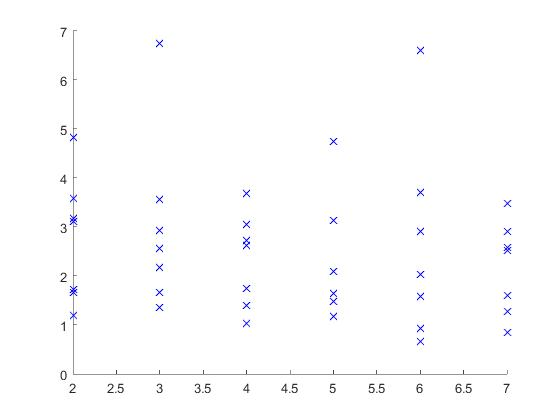
\includegraphics[width=1\textwidth]{ez_overlap_prox_false.jpg}
                	\end{minipage}
                	\caption{Effect of enforcing a larger minimum overlap on EZ's RGEA with respect to percentage of correctly identified proximate points (left, red) and the number of falsely identified proximate points per correct point (right, blue).}
                \end{figure}
                
                \begin{figure}[h]
                	\label{fig:ez_prox_prox}
                	\centering
                	\begin{minipage}{0.5\textwidth}
                		\centering
                		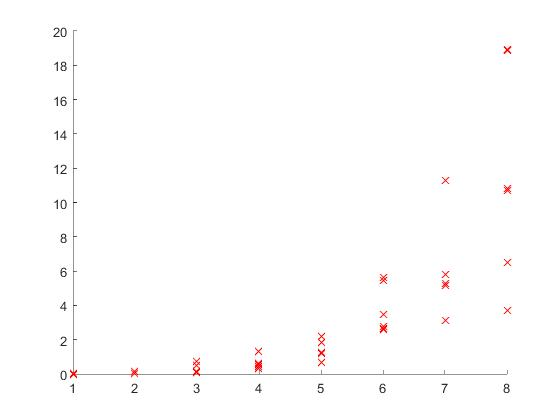
\includegraphics[width=1\textwidth]{ez_prox_prox_correct.jpg}
                	\end{minipage}\hfill
                	\begin{minipage}{0.5\textwidth}
                		\centering
                		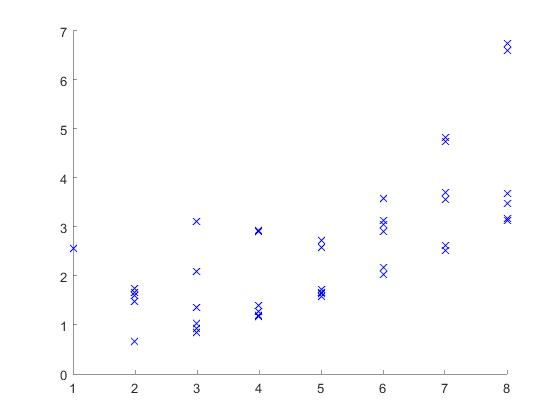
\includegraphics[width=1\textwidth]{ez_prox_prox_false.jpg}
                	\end{minipage}
                	\caption{Effect of increasing the proximity threshold on EZ's RGEA with respect to percentage of correctly identified proximate points (left, red) and the number of falsely identified proximate points per correct point (right, blue).}
                \end{figure}
                
                First to be discussed are the results of running EZ's RGEA over the data set while tuning the \texttt{prox\_threshold} and \texttt{min\_AP\_overlap} parameters. As shown in figure \ref{fig:ez_overlap_prox}, imposing a greater restriction on the minimum number of APs visible at both points to be considered had a minimal impact on the algorithms performance, even when only 1 common AP is required. This is likely due to the other restrictions over set comparison imposed in section \ref{sec:dataprep} rendering this metric less useful for accuracy. Profiling also revealed no significant change in run-time despite the reduction in calculations required. However, it is anticipated that this is due to the slow performance of Matlab's \texttt{ismember} function and could likely be improved with a more efficient comparison function.
                
                As was anticipated however, increasing the average RSSI difference threshold at which points are deemed proximate enforced a very strong relationship between the number of points correctly and falsely identified. What was not anticipated however was the rapid increase in correct-to-false ratio. The results shown in figure \ref{fig:ez_prox_prox} highlight a rapid increase in inclusion when the threshold is set above 5dB, including up to 5 times more correct results but up to 7 times more falsely proximate points than those extra valid results. The effect of increasing this threshold is theoretically simple, but the reason behind the sudden increase could result from a number of factors such as the inclusion threshold including some new devices directly rather than transitively. \citet{chintalapudi2010indoor} recommended a value of 3dB in their experiments at which ``RGEA estimates receiver gain differences accurately within 1-3dB''. This claim will be verified with subsequent testing in section \ref{sec:gainestimation}.
                
                Unfortunately, the extreme run-time of computing pair-wise similarity over the whole data set in combination with some unanticipated interruptions to experimentation lead to a very truncated data set from the heuristic evaluation (as shown in figure \ref{fig:h_prox_summary}). However, even from this small collection of points, some obvious conclusions can be drawn; first being the tremendous number of falsely proximate pairs. In the worst case, the heuristic RGEA is identifying 18 incorrect pairs for every 1 correct, more than 2.5 times that of the worst observed for EZ's method. However, the second point of note is that the heuristic method also finds 2.5 times more of the correct pairings, over 50\% in some cases. It should be noted though that the total number of potential pairs given the 19,000 strong data set is roughly 180,500,000, so the algorithm is still far from selecting every pair.
                
                \begin{figure}
                	\label{fig:h_prox_summary}
                	\centering
                	\begin{tabular}[h]{| c | c | c | c | c |}
                		\hline
                		\texttt{min\_AP\_strength} & \texttt{min\_strong\_overlap} & Correct & Missed & False \\ \hline
                		-100 & 2 & 66,406 & 63,284 & 1,200,000 \\
                		-100 & 3 & 25,803 & 103,890 & 329,010 \\
                		-90 & 2 & 66,118 & 63,572 & 1,186,700 \\
                		-90 & 3 & 25,734 & 103,960 & 327000 \\
                		-80 & 2 & 59,055 & 70,635 & 1,030,300 \\
                		-80 & 3 & 23,707 & 105,980 & 289,420 \\ \hline
                	\end{tabular}
                	\caption{Experimental results from heuristic proximity checking with \texttt{num\_strong\_APs} set to 4}
                \end{figure}
                
                Upon further investigation into the set of false pairs, it was found that significant number of pairs taken on different floors with over 10 meters lateral difference between them had almost identical maximal sets and an average difference of 2dB for each common maximum RSSI measurement, breaking the assumption made before testing. This type of accidental pairing would seem unavoidable according to the techniques employed here and as such a brief experiment was run to evaluate performance on the data set separated into the 2D subspaces across which modelling would be performed. Promisingly the heuristic algorithm identified the exact same set of correct pairs with a 20\% reduction in false-positives for parameters (\texttt{min\_AP\_strength}: -100, \texttt{min\_strong\_overlap}: 3). This bring's estimated performance in line with EZ's RGEA but reduces run time by roughly 25\%. While seemingly unreasonable (especially for any system relying directly on correct identification of proximate pairs), the impact of these excess points will now be evaluated in section \ref{sec:gainestimation}'s gain estimation experiments.
		    
		    \subsection{Relative Gain Estimation}
		    \label{sec:gainestimation}
            
                Ultimately, the amount of correctly estimated gain between pairs of devices is the best measure of the proximity metric's performance in this context. As discussed previously, both techniques find a disproportionately large number of falsely proximate pairs for each one correctly identified. This experiment will judge the extra included points' impact on the actual result by calculating the amount of relative gain identified when using these sets of `proximate' points. In order to test the validity of the application of these techniques over a number of spaces, each technique (and combination of parameters) will be run over the UJIIndoorLoc data set split into the 2D subspaces that will be used for modelling. The techniques will then be judged by their averaged performance over all spaces (for the best general-fit parameters) according to the percentage error of the total existing relative gain across all device pairs that they identify (calculated through the ground truth estimator).
                
                \begin{figure}[h]
                    \label{fig:ez_comp}
                    \centering
                    \begin{minipage}{0.5\textwidth}
                        \centering
                        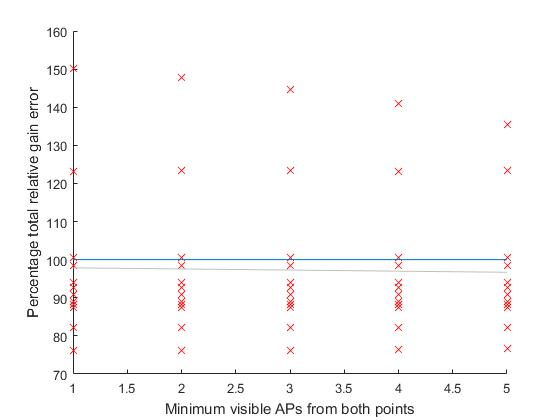
\includegraphics[width=1\textwidth]{ez_overlap.jpg}
                    \end{minipage}\hfill
                    \begin{minipage}{0.5\textwidth}
                        \centering
                        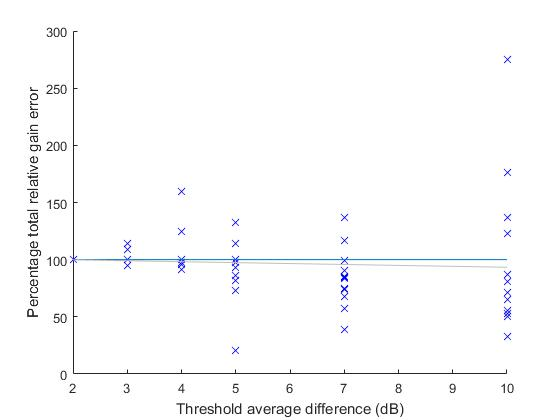
\includegraphics[width=1\textwidth]{ez_prox.jpg}
                    \end{minipage}
                    \caption{Effect of changing EZ's RGEA parameters on percentage of missed relative gain.}
                \end{figure}
                
                First to be evaluated again are EZ's RGEA parameters. The graphs shown in figure \ref{fig:ez_comp} show the impact of tuning each parameter on the percentage total relative gain error. Each point shows the percentage total relative gain error for a 2D subspace, averaged for all potential values of the other parameter (assuming parameter independence). The blue line shown at 100\% shows the reference amount of gain error if no calculation were applied, while the grey line shows trend relating to tuning the parameter across all subspaces.
                
                In line with the results from section \ref{sec:prox_est}, increasing the minimum number of APs visible from both points in a potential pair appears to have no effect on the accuracy of the algorithm; maintaining roughly the same average and standard deviation of gain errors. Allowing a larger difference in gain's for proximate points however has a marked increase in potential to correctly recognise gain differences between devices. The greatest increase in performance is seen at around 7dB, where the majority of spaces had their gains corrected by roughly 30\% as opposed to EZ's claim that 3dB provided the best results. Increasing the gain threshold further appears to slightly decrease the median gain error, but the standard deviation takes a significant hit, potentially increasing the gain error by up to 150\%. When comparing these results to those found in the proximity experiments, the inclusion of more proximate pairs explains the increase in potential gain identified and those included erroneously seemingly bias the estimated gain towards $0$dB in the majority of cases, making EZ's gain estimation pessimistic, but safe.
                
                \begin{figure}[h]
                    \label{fig:h_minAP}
                    \centering
                    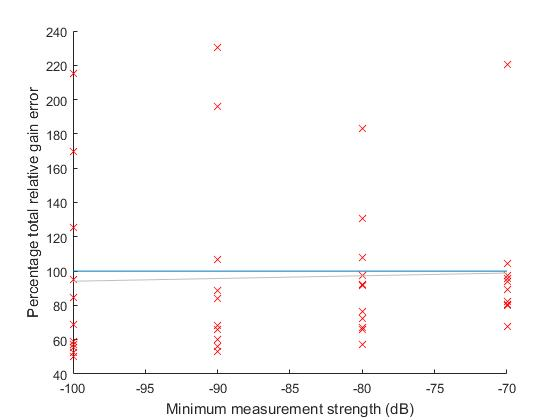
\includegraphics[width=0.6\textwidth]{h_minAP.jpg}
                    \caption{Effect of increasing the minimum measurement strength required for heuristic RGEA on percentage of missed relative gain.}
                \end{figure}
                
                The results of testing the heuristic RGEA's performance however are much harder to analyse because of the strong relationship between \texttt{min\_strong\_overlap} and \texttt{num\_strong\_APs}. It is assumed though that \texttt{min\_AP\_strength} will have an independent effect over the accuracy of the algorithm and it's affect is displayed in figure \ref{fig:h_minAP}. Similar to the results shown in \ref{fig:h_prox_summary}, reducing the set analysed by imposing a minimum threshold reduces the number of pairs included globally and in correlation, the amount of gain that can be derived (as shown by the distribution clustering towards 100\% error with increased threshold).
                
                \begin{figure}[h]
                    \label{fig:h_overlap}
                    \centering
                    \begin{minipage}{0.5\textwidth}
                        \centering
                        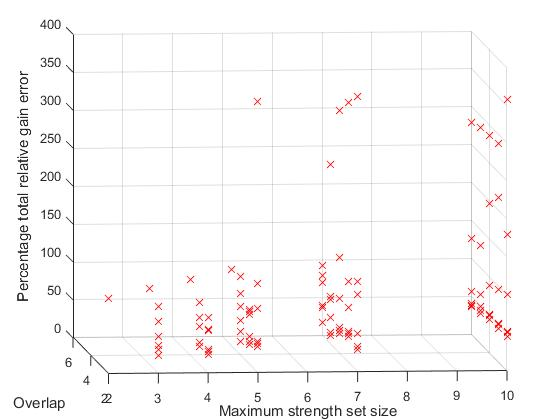
\includegraphics[width=1\textwidth]{h_overlap.jpg}
                    \end{minipage}\hfill
                    \begin{minipage}{0.5\textwidth}
                        \centering
                        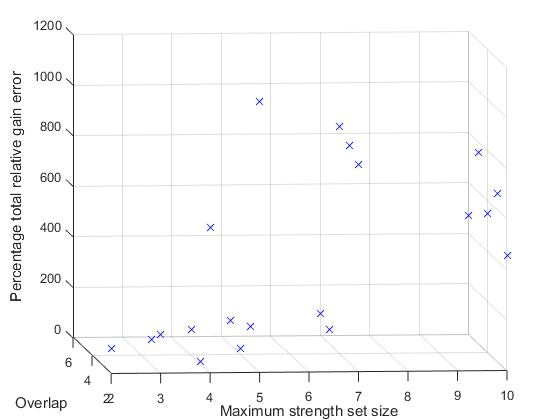
\includegraphics[width=1\textwidth]{h_overlap_anomalous.jpg}
                    \end{minipage}
                    \caption{Effect of changing heuristic RGEA's maximal set parameters on percentage of missed relative gain. General distribution shown in red (left) and the anomalous subspace in blue (right).}
                \end{figure}
                
                Shown in figure \ref{fig:h_overlap} is the relationship between the maximal set size and overlap (\texttt{num\_strong\_APs} and \texttt{min\_strong\_overlap}), and their effect on relative gain error. These results have had to be split because of the extreme outliers produced by one particular subspace (whose results are shown in blue on the right). In the worst case, this space produced 3 times more error than the rest of the data set with unknown cause and as such have been excluded to make the results of the general case clearer.
                
                As was theorised in section \ref{sec:dataprep}, requiring the maximal set to overlap entirely produced no proximate points and as such no gain estimation. For small maximal sets (<5) however, allowing for a single difference between the sets provided extremely accurate estimations, with errors as low as 10\% total gain missed. Surprisingly, these results run contrary to the implied errors that could have arisen from the seemingly poor proximity estimation displayed in figure \ref{fig:h_prox_summary}. This implies that the proximity estimation displayed through using heuristic RGEA is more of a fingerprinting method, marking all points in a larger area, but in a way such that the errors caused by pairing points on opposite sides of the zone are balanced out overall. However, when these fingerprinting zones are set too large (>5), with too little overlap required (>2 less than the size of the set), the accuracy of the gain estimation drops significantly with much less certainty towards the outcome. 
                
                To summarise, EZ's RGEA's reported accuracy was not reproducible, despite testing a wide range of parameters. Heuristic RGEA however was demonstrated to reliably calculate a significant amount of the existing relative gain across 2D spaces by comparing fingerprinted zones. As a result, the recommended parameters for heuristic RGEA are \texttt{min\_AP\_strength}: -100, \texttt{num\_strong\_APs}: 4, \texttt{min\_strong\_overlap}: 3. Estimation over the whole data set was tested, but the results are excluded because of the extreme skew provided by the inclusion of results from the anomalous subspace shown in figure \ref{fig:h_overlap}.
	    
	    \section{Modelling Accuracy}
	    \label{sec:modeleval}
        
            In this section, the IPS will be evaluated as a whole against it's potential to localise data points in a 2D space. These results will aim to validate the decisions made in section \ref{sec:modelcreation}, the theoretical assumptions made behind those decisions and the results boasted by \citeauthor{chintalapudi2010indoor}'s implementation \citep{chintalapudi2010indoor}.
            
            The `localisability' of each model is split into two metrics: the median distance error between the sets of estimated and actual locations of the test data points and the percentage of the test data points that are localisable within the modelled space. To this end, the UJIIndoorLoc data set is already split into source and test data subsets for techniques relying on the modelling data set to cover the entirety of the space under test such as this \citep{torres2014ujiindoorloc}. While having pre-defined test data sets removes the random factor normally associated with testing machine learning techniques, the fact that UJIIndoorLoc can be split into a number of independent 2D subspaces increases the validity of these experiments by taking the average performance over multiple environments rather than a randomly chosen subset of the same environment.
            
            \begin{figure}[h]
                \label{fig:datapoints}
                \centering
                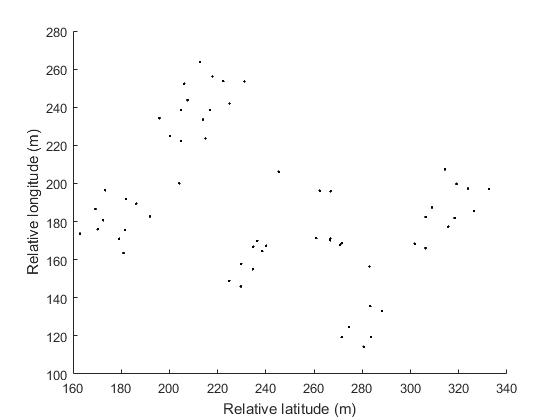
\includegraphics[width=0.6\textwidth]{datapoints.jpg}
                \caption{Sample data point distribution for a single floor of a building from the UJIIndoorLoc data set \citep{torres2014ujiindoorloc}.}
            \end{figure}
            
            It should be noted however that UJIIndoorLoc is not the ideal data set for testing EZ's modelling technique, merely the most complete and publicly available set for starting a framework in line with the project's goals. As shown in figure \ref{fig:datapoints}, samples were generally taken at the entrances to each logical space (i.e. rooms), but this fails to represent the majority of traffic along corridors or distributed across larger open spaces. While it can be argued that the greatest impact on signal strength across a number of smaller rooms (such as an office environment) will be the walls (as modelled by RADAR's wall attenuation factor \citep{bahl2000radar}) and as such measurements within each space should have little variation, a truly organic data set gathered through crowd-sourcing would provide the most ecologically valid results.
            
            \subsection{Thresholding and Localisation}
            
	            The first component to be evaluated is the last component of the system: the modeller itself as this establishes a base-line around which any additions can be judged. As discussed previously, this experiment will demonstrate the average performance of the modeller over the set of 2D subspaces available in the UJIIndoorLoc data set with respect to any minimum RSSI threshold applied and the localisation technique used (see section \ref{sec:modelcreation}). The input data will assume the role of a sample data set; gathered with all data point locations known before modelling as to avoid employing AP propagation and provide a `best-case' scenario. No RGEA or other data preparation will be employed however as no actual ground truth values are provided, so the experiment avoids introducing any other sources of potential error.
            
                \begin{figure}[h]
                    \label{fig:threshold}
                    \centering
                    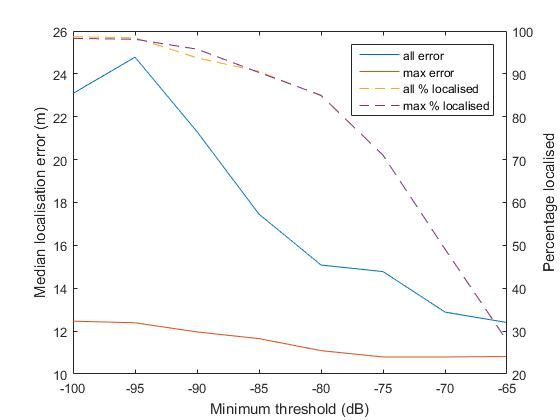
\includegraphics[width=0.6\textwidth]{threshold.jpg}
                    \caption{Effect of increasing the minimum RSSI strength required on the localisability of a given space.}
                \end{figure}
                
                Figure \ref{fig:threshold} shows the benefit of taking advantage of the thresholding and maximum strength trilateration techniques described in section \ref{sec:modelcreation}. As anticipated, attempting to localise a data point based on every parameterised AP produced a large number of conflicting constraints as a single low-strength measurement carries the same weight as any one more likely reliable measurement of a higher-strength. Reducing the impact of low strength measurements through thresholding proves most effective at around -80dB, showing a reduction in error of roughly 30\% (8m) while maintaining >80\% coverage of the space. Increasing the threshold further however shows diminishing returns on error reduction at the cost of a rapidly decreasing coverage.
                
                Much more effective than reducing the set of RSSIs used for modelling though was reducing the set of RSSIs per point used for localisation. The results gathered in figure \ref{fig:threshold} show that restricting localisation of data points to the strongest 3 observed RSSIs reduces the median localisation error by just under half at no cost to the amount of localisable space. Thresholding in conjunction with this technique does still show an improvement by refusing to localise less reliable measurements when modelling, but provides much less significant 12\% (1.5m) reduction in error for the same penalty to localisable space.
                
            \subsection{Solution Space Exploration}
                
                Following the success of the maximum strength localisation technique, a second experiment was devised to assess the impact of using simulated annealing over the full genetic algorithm specified by \citet{chintalapudi2010indoor}. In this experiment, the modeller was run over the same set of subspaces with no minimum RSSI threshold using the same maximum strength localiser, but the simulated annealer was allowed to run 100 times when modelling and select the best result as opposed to only enforcing a minimum fitness as defined in section \ref{sec:modelcreation}. The objective here is to emulate the number of solutions explored by a full genetic algorithm and show how an improved fitness for each AP would affect the accuracy of the models in the general case.
                  
                \begin{figure}
                    \label{fig:uber}
                    \centering
                    \begin{tabular}[h]{| c | c | c | c |}
                        \hline
                        Building ID & Floor ID & Minimum (m) & 100 runs maximum (m)  \\ \hline
                        0 & 0 & 8.17 & 9.19 \\
                        0 & 1 & 10.94 & 10.75 \\
                        0 & 2 & 7.97 & 13.45 \\
                        0 & 3 & 7.59 & 10.42 \\
                        1 & 0 & 10.9 & 9.91 \\
                        1 & 1 & 12.97 & 14.25 \\
                        1 & 2 & 18.57 & 16.5 \\
                        1 & 3 & 12.37 & 10.22 \\
                        2 & 0 & 21.72 & 14.72 \\
                        2 & 1 & 10.2 & 11.62 \\
                        2 & 2 & 13.2 & 16.74 \\
                        2 & 3 & 14.96 & 11.28 \\ \hline
                        \multicolumn{2}{| c |}{Mean} & 12.46 & 12.42 \\ \hline
                    \end{tabular}
                    \caption{Localisation error comparison between a minimum fitness simulated annealer and 100 runs selecting the best fit to the modelling data. Both runs created models localising 98\% of test data points.}
                \end{figure}
                
                The results in figure \ref{fig:uber} show that while the average case accuracy of the extended run does not show any significant change, the standard deviation of the error does decrease, meaning that any single extended run is likely to be more accurate in the general case but the constraints applied in section \ref{sec:modelcreation} avoid the faster modelling techniques generating significantly worse models. This result is positive when evaluated against the project's goals as it demonstrates that a representative set of parameters can be generated even with a much shorter modelling phase (up to 100 times faster), allowing for more combinations of techniques to be evaluated in a short period.
	    
		    \subsection{Clustering Effectiveness}
            
                Given the increased data set size and area under observation compared to those demonstrated by \citet{chintalapudi2010indoor}, it was noted in section \ref{sec:datacluster} that the use of hierarchical clustering over the UJIIndoorLoc data set might eliminate bias and reduce the modelling time when compared against modelling all observations. As such, this experiment is designed to represent the changes imposed on the generated model through the implementation of APSelect and LocSelect. To avoid over experimentation, each form of APSelect and LocSelect will be applied to the most interesting parameters of the previous experiment, most notably the threshold levels of -100 and -80 dB on both localisation techniques. Metrics reported will be the \% of APs observed before thresholding is applied that are parameterised by the finished model and the same localisability metrics from the previous section to demonstrate impact on the model's accuracy.
            
                \begin{figure}
                    \label{fig:apselect}
                    \centering
                    \begin{tabular}[h]{| L | L | c | c | L | c | c | L |}
                        \hline
                        \multirow{2}{*}{\parbox{2cm}{\centering \vspace{.6\baselineskip} Localisation Method}} & \multirow{2}{*}{\parbox{2cm}{\centering \vspace{.6\baselineskip} APSelect Type}} & \multicolumn{3}{c |}{-100dB Threshold} & \multicolumn{3}{c |}{-80dB Threshold} \\ \cline{3-8}
                        & & \% APs & \% Loc & Avg. Med. Err. (m) & \% APs & \% Loc & Avg. Med. Err. (m) \\ \hline
                        \multirow{3}{*}{EZ} & None & 100 & 98 & 22.5 & 54 & 86 & 15.1 \\
                        & Overlap & 25 & 87 & 22.4 & 19 & 58 & 16.4 \\
                        & Max & 77 & 96 & 23.7 & 40 & 72 & 16.6 \\ \hline
                        \multirow{3}{*}{Heuristic} & None & 100 & 99 & 11.9 & 54 & 85 & 11.1 \\
                        & Overlap & 25 & 91 & 16.7 & 19 & 56 & 15.7 \\
                        & Max & 77 & 98 & 14.8 & 40 & 72 & 13.1 \\ \hline
                    \end{tabular}
                    \caption{Impact of using different variants of the APSelect algorithm on model size and accuracy, averaged across all tested subspaces.}
                \end{figure}
                
                Figure \ref{fig:apselect} shows the average results of multiple runs of this experiment over each 2D subspace with differing combinations of the APSelect and localisation components. In \citeauthor{chintalapudi2010indoor}'s study, only the first two results of the -100dB threshold column were evaluated and their findings are replicated here. When using the EZ localisation scheme and overlap APSelect algorithm, the size of the model can be reduced by over 75\% for minimal penalty to localisability. However, when APSelect is run over the heuristic (maximal) localisation scheme, the lack of model completeness significantly reduces the median accuracy. 
                
                Similarly, reducing the number of parameterised APs through both thresholding and APSelect appears to reduce the accuracy of the new model. It is noteworthy though that thresholding is only a linear operation, where hierarchical clustering is significantly more complex. Thus it would seem that the APSelect is much less useful when applied generally as the only result benefiting from its inclusion is the most basic EZ implementation. 
                
                While the heuristic APSelect appears to perform more favourably with respect to localisability, this is likely due to it less efficiently identifying redundant APs as its application to the most basic localisation technique actually increases error with less APs removed. Unfortunately, the heuristic clustering mechanism appears to be less efficient as a whole as it was originally intended to add a small decision overhead to avoid performing large redundant calculations. However, this 4-value set intersection check in Matlab has a much longer run time than performing the actual 520-value calculation and as such decreases the performance of each check significantly.
                
                This was intended to make LocSelect over larger data sets more feasible; as explained in section \ref{sec:datacluster}, the pairwise similarity checking behind hierarchical clustering grows in complexity rapidly enough that LocSelect over 1,000 data points was rendered computationally intractable. However, due to a number of interruptions to the experimentation environment and the unexpected poor performance of the heuristic approximation, no results were able to be gathered to demonstrate the effectiveness of LocSelect, though it is theorised it may improve the accuracy of the model by removing bias towards any one heavily measured location.
        
        \section{Summary}
        
            This chapter has demonstrated the combined and individual performances of each component part of the EZ IPS and their variants in both their IPS application and general purpose performance where applicable. The accuracy of models created using the original EZ components was shown to degrade over large, irregular data sets such as UJIIndoorLoc compared to the initial statistics gathered by \citet{chintalapudi2010indoor}, but using the simple modifications developed in this project, a significant improvement was shown and recommended parameters were extracted (a copy of the software under test is made available on GitHub \citep{git}).
            
            While the components were tested in order to verify \citeauthor{chintalapudi2010indoor}'s findings and to provide a base-line against which future techniques can be compared, the UJIIndoorLoc data set was also briefly evaluated for its validity under test \citep{torres2014ujiindoorloc}. The fact that the 3D space could be broken down into a number of 2D subspaces for validation of general purpose performance was a major positive, but the distribution of data points was found to be less representative of a set of measurements that might be gathered through natural crowd-sourced movements. This combined with the lack of indication of GPS visibility highlighted the need for a truly crowd-sourced data set for the most ecologically valid evaluation as while a random removal of modelling data locations might seem like an adequate emulation, over a data set of this size it is unlikely that AP propagation would be stimulated for any models with representative coverage.
	
	\chapter{Conclusion}
    \label{chap:conclusion}
    
        This final chapter will review the work carried out over the life cycle of the project and identify a set of potential further work topics. As the initial set of project aims were relatively broad, the literature review in chapter \ref{chap:related} was necessary to explore the set of deliverables that this project could focus on. The review itself showed how the combined fields of crowd-sourcing, indoor positioning and automated floor planning that might make up a building analytics framework are diverse, continually growing but seemingly disjoint with no studies looking into their combined power and the effectiveness thereof. With no common comparison points between systems even within the same field, the necessity of an evaluation framework was further exemplified.
        
        In chapter \ref{chap:problem}, the solution space was then reviewed and a starting point identified. While the whole building analytics framework was deemed to be of too grand a scale for a one man project, it was foreseen that each component could be developed independently by a small team and combined at a later date. From here, it was thought that the most useful first component to build would be an indoor positioning system as it would provide the largest base around which to build the other components and techniques in future studies. Of the surveyed IPS techniques, the EZ IPS components were selected as being most in line with the project aims, requiring no prior knowledge of the building being modelled, consisting of modular components viable for re-use and experimentation alongside other techniques, and being able to make use of the freely available UJIIndoorLoc data set for comparisons against future work \citep{chintalapudi2010indoor, torres2014ujiindoorloc}.
        
        With no reference implementation available, chapter \ref{chap:method} set about creating one for use as part the future framework. With a different set of goals in mind, creating a new version proved advantageous, allowing for a different set of design decisions including implementation language and general structure. Implementing based on EZ's specification alone however proved to be problematic, with numerous edge cases, details left unspecified and requiring a number of fixes to make the system compatible with a 1,000 reading data set (more representative of a crowd-sourced scenario) as opposed to the 101 tested \citep{chintalapudi2010indoor}. Along with the fixes, a number of heuristic approximations were devised to reduce run-time complexity while maintaining performance over larger data sets, primarily based around quick and cheap focussing on more reliable RSSI values.
        
        Finally, a comprehensive series of tests was run over this project's implementation in chapter \ref{chap:eval}. As this project is looking to have techniques and components re-used in other applications, the general purpose performance of each part was considered as well as its application as part of the IPS (see proximate point identification and relative gain estimation in section \ref{sec:rgeaeval}). While general purpose performance proved poor, the application of simple heuristic techniques in tandem with the principles garnered from EZ performed amicably, with localisation errors of <10\% of the space modelled in a much shorter time frame than EZ's 7+ hours. The suitability of the data set used was also evaluated and found to be less than optimal, but useful as an initial comparison point.
        
        These results of course are not anticipated to compete with state-of-the-art given the diversity of potential techniques to be applied and results from other studies showing that techniques such as Horus attain the highest accuracy when given much more thorough data sets \citep{youssef2005horus, chintalapudi2010indoor}. Though the implementation devised in this project is roughly half as accurate as that reported by \citet{chintalapudi2010indoor}, this is likely due to the less regular spacing of the data set gathered by \citet{torres2014ujiindoorloc} and the fact that \citeauthor{chintalapudi2010indoor} did not test over a data set of this size. However, given the lack of reference implementations for many of these techniques, the project goal of encouraging collaborative development towards a comprehensive building analytics framework has been achieved through the identification of comparable techniques, a data set and metric to compare them by and providing a reference implementation around which to build.
        
        Given the developmental nature of the overarching project aims, there are still several pieces of short-term work to be done before this could truly be considered a framework. The first of which would be the creation of a truly crowd-sourced data set. This would likely need to be backed up by regularly spaced sample readings with ground truth locations across the space, but given a complete set of sensor readings with total coverage might help to identify at what locations each sensor can be relied upon. For example, in the UJIIndoorLoc data set it is unknown as to at which point GPS signal is lost and so incomplete data set tests were unlikely to be representative. The application of techniques developed here on this new data set would also help to verify performance comparisons in other future works.
            
        The second would be some implementation of an automated floor plan generator as discussed in section \ref{sec:floorplans}. Using a data set with a more completely defined environment (such as that promised by \citet{JoaquinEmail}), comparison between theoretical models generated and the ground truth behind them would be possible, potentially paving the way for a representative comparison metric to be developed.
            
        With at least one of every component in place, more long term comparisons could then be developed, evaluating techniques and combinations thereof to identify more situational strengths and weaknesses. Particular cases that could be taken advantage of might be edge-case APs (such as those shown in figures \ref{fig:fringe} and 4.5) to aid with immediately recognising small areas or using the fact that an AP is not visible to take into account when defining likelihood of a particular location. These in combination with a Horus-style fingerprinting of the space could lead to extremely precise localisation by recursively eliminating unlikely locations, but it could ultimately be one of the largest indoor positioning systems (in terms of complexity) to date.

        One final foreseeable extension to current techniques is that of the third dimension. Theoretically, when applied to EZ, an extra parameter for elevation of access points and data points should only require one extra observation to uniquely determine. While this could be approximated through use of stacked 2D spaces, for a truly 3D approach a data set in kind would also need to be gathered for technique comparison. Only once a 3D space of significant size can be efficiently monitored, localised and mapped with no significant human effort will this framework truly be considered complete.
        
    \bibliography{report.bib}
	
\end{document}
